%%%%%%%%%%%%%%%%%%%%%%%%%%%%%%%%%%%%%%%%%%%%%%%%%%%%%%%%%%%%%%%%%%%%%
% Richard Boardman rick@ic.ac.uk
% PhD Thesis - Department of Electrical and Electronic Engineering
% Imperial College London SW7 2BT UK
% %%%%%%%%%%%%%%%%%%%%%%%%%%%%%%%%%%%%%%%%%%%%%%%%%%%%%%%%%%%%%%%%%%%
% Improving Tool Support for Personal Information Management
% CHAPTER 3 - LITERATURE REVIEW
% Version 25, 10th November 2003
%%%%%%%%%%%%%%%%%%%%%%%%%%%%%%%%%%%%%%%%%%%%%%%%%%%%%%%%%%%%%%%%%%%%%
%%%%%%%%%%%%
%% VOCAB
%%%%%%%%%%%%
%% Good words for review: appraise, examine, consider, assess previous work, scrutinise, acknowledge}
%% Good words for analysis: it has been argued/proposed, justify, suggest, compelling}
%% suggests that X leads to Y
%% implications for Y are discussed
%% phrase: used to argue the potential
%%%%%%%%%%%%%%%%%%%%%%%%%%%%%%%%%%%%%%%%%%%%%%%%%%%%%%%%%%%%%%%%%%%%%%%%%%%%%%%%%%%%%%
%% AIm: produce a well-thought out  criticism of:
%% a) why important
%% b) how it affected my work
%% c) present evolution of ideas in my field
%% d) how the problem addressed in this thesis relates to them
%%%%%%%%%%%%%%%%%%%%%%%%%%%%%%%%%%%%%%%%%%%%%%%%%%%%%%%%%%%%%%%%%%%%%%%%%%%%%%%%%%%%%%
%% Use CF to structure?
%% Relate sections to parts of thesis where used
%% Consider previous research in terms of quality and validity 
%%%%%%%%%%%%%%%%%%%%%%%%%%%%%%%%%%%%%%%%%%%%%%%%%%%%%%%%%%%%%%%%%%%%%%%%%%%%%%%%%%%%%%

%%%%%%%%%%%%%%%%%%%%%%%%
\section{Introduction}
\label{review-introduction}
%%%%%%%%%%%%%%%%%%%%%%%%
This chapter offers a critical review of prior research relevant to Personal Information Management (PIM). %\footnote{This draft of ``Chapter 3 Literature Review'' was printed \today}.
% Existing knowledge is surveyed from the field of Human Computer Interaction (HCI) and other related disciplines such as Information Science and Cognitive Psychology.  A particular focus is taken on Human-Computer Interaction, since this is the field to which the author seeks to contribute.
%%%%%%%%%%%%%%%%
%% ADD DISCLAIMER
%%%%%%%%%%%%%%%%
% It should be noted that the interdisciplinary nature of research, and the broad range of design in this area, plus lack of coherency means that any survey of work cannot hope to be complete. However it is hoped that a representative summary of important work is provided. 
%%%%%%%%
% AIMS
%%%%%%%%
%% link from research gap to the specific problem
%% identify areas in need of further research
%% present context of the work
%%
%% Identify research gaps which this thesis can address}
%% 
%% after stating how existing knowledge is lacking for solving this problem.
%% 
%% review concludes by attempting to provide justification/motivate/argue for my chosen methodology and contributions.
% field evidence to justify the design and methodological decisions made
%%%%%%%%%%%%%%%%%%%%%%%%%%%%%%
% Relate to overall PhD aims
%%%%%%%%%%%%%%%%%%%%%%%%%%%%%%
% The chapter offers three contributions towards the overall thesis. Firstly the chapter aims to review previous work in the field in terms of key contributions and limitations.
%%%%%%%%%%%%%%%%%%%%%%%%%%%%%%%%%%
% \subsection{Overview of Chapter}
%%%%%%%%%%%%%%%%%%%%%%%%%%%%%%%%%%
% The chapter is structured as follows.
Firstly, \textbf{Section~\ref{review:hci}} provides an overview of Human-Computer Interaction (HCI), the research field to which the thesis contributes.
% PIM is identified as an important application domain within HCI.
\textbf{Section~\ref{review:pim-research-overview}} identifies the three main types of HCI research related to PIM: empirical studies, technology prototypes, and theory development.  The next three sections deal with each area in turn.  \textbf{Section~\ref{review:pim-empirical-review}} reviews empirical work, \textbf{Section~\ref{review:pim-technological-review}} surveys PIM technology, focusing on design efforts to improve PIM-integration, and \textbf{Section~\ref{review:pim-theory-review}} reviews relevant theory.
% A second aim is to identify gaps in current knowledge where further work is required, and where this thesis can contribute.
% summarizes their main findings and discusses how they relate to one another.  The section also makes recommendations for more effective future research in the area.
% Based on this critical analysis of prior work, a research agenda will be laid out to address the identified research problem.
% A final aim is to justify the selection of methodology . This involves the surveying of methods and techniques applied to the area, as well as others that could be applied.
%  sets out a research agenda that defines the initial plan of work taken in this thesis.
% Finally \textbf{Section~\ref{review:conclusion}} summarizes the contributions of the chapter towards the overall thesis.
\textbf{Section~\ref{review:discussion}} draws together the three areas, and identifies a key research gap, the lack of empirical support for the design of PIM-integration mechanisms.  Based on this analysis, \textbf{Section~\ref{review:research-agenda}} sets out a research agenda for the thesis, and \textbf{Section~\ref{review:methodology}} justifies the selection of methodology employed in later chapters. % in the thesis.







%%%%%%%%%%%%%%%%%%%%%%%%%%%%%%%%%%%%%%%%%%%%%%%%%%%%
%%%%%%%%%%%%%%%%%%%%%%%%%%%%%%%%%%%%%%%%%%%%%%%%%%%%
\subsection{Human-Computer Interaction}
\label{review:hci}
%%%%%%%%%%%%%%%%%%%%%%%%%%%%%%%%%%%%%%%%%%%%%%%%%%%%
%%%%%%%%%%%%%%%%%%%%%%%%%%%%%%%%%%%%%%%%%%%%%%%%%%%%

%%%%%%%%%%%%%%%
% SIGNPOSTING
%%%%%%%%%%%%%%%
% This section provides an overview of Human-Computer Interaction (HCI), the research field to which the thesis contributes. The Task-Artefact cycle is presented as a framework in which HCI research and practice can be discussed. Personal information management is considered as a key application domain within HCI.

%%%%%%%%%%%%%%%%%%%
% Intro to HCI
%%%%%%%%%%%%%%%%%%%
%% Sutcliffe's framework of HCI application and technology domains is discussed. 
%% 
%% HCI is a young, interdisciplinary, applied research field containing many competing methods and research paradigms.  The chapter commences with a broad overview/sketch of the aims of HCI, its dominant research paradigms, and the various forms that HCI knowledge can take.  This overview is used to structure the remainder of the chapter focused on personal information management.
%%
%% The aim of HCI research is to provide a knowledge base to support  directed at the design of usable interactive systems~\citep{sutcliffe:00}.
%% Sutcliffe terms "`HCI-research"' as "`HCI theory"'
%% research theory versus craft-level experience/heuristics
%%  NB HCI-research can also  (those directed at research and those directed at design)
\citet{acm:96} define Human-Computer Interaction (HCI) as the \textit{``discipline concerned with the design, evaluation and implementation of interactive computing systems for human use and with the study of major phenomena surrounding them''}.
%% Two aspects of HCI exist: HCI research and HCI practice, differentiated by their end-product.
A key aim of HCI research is to provide a knowledge base to guide the design of interactive systems.  % Thus the end-product of HCI research is knowledge, whilst the end-product of HCI practice is the design of interactive systems. To confuse the picture, much HCI research is concerned with the design of interactive systems -- using the same design methods as HCI practice.
% \textbf{Figure~\ref{fig:chapter2_hci_overview}} provides a graphical summary of HCI.  HCI research draws on a range of ``foundational'' disciplines such as psychology and sociology, that provide theories and methods for the study and development of interactive systems.
%% THINK: science/discipline/field/area/issues}.
% %%%%%%%%%%%%%%%%%%%%%%%%%%%%%
% FIGURE - Overview of HCI
%%%%%%%%%%%%%%%%%%%%%%%%%%%%%%%
%\begin{figure}[hbtp]
%	\begin{center}
%		\leavevmode
%		\includegraphics[width=.9 \textwidth]
%		{pictures/research_review/Ch2-OverviewOfHCI.pdf}
%	\end{center}
%	\caption{Human Computer Interaction: an epistemological overview}
%	\label{fig:chapter2_hci_overview}
%\end{figure}
%%%%%%%%%%%%%%%%%%%%%%%%%%%%%%%%
% Products of HCI research
%%%%%%%%%%%%%%%%%%%%%%%%%%%%%%%%
%% CITE: methodological and substantive (REF).
%% Broadly speaking, methodological contributions to knowledge are concerned with \textit{how} to perform design and further research and consists of methods, heuristics and techniques.
%% Substantive contributions to knowledge consists of specific research findings such as designs, their evaluations, and study findings.
% -- all concerned with \textit{how} to design interactive systems and to pursue research into their usage
% Newman~\citep{newman:94} identifies a range of contributions from HCI research.
The output of HCI research includes two types of knowledge: (1) substantive, and (2) methodological.  Substantive knowledge documents the results of research and may include experimental accounts, the designs of interactive systems and techniques, and models and theories of user behaviour. Methodological contributions offer guidance for future research and design in terms of heuristics, tools and methods.

%%%%%%%%%%%%%%%%%%%%%%%%%%%%
% The task-artefact cycle
%%%%%%%%%%%%%%%%%%%%%%%%%%%%
%% \textit{The cycle can be se as framework for discussing practice and research: both HCI research and HCI practice can be mapped onto the cycle.} 
%%
%% Although the cycle does not directly encompass theory-building, the output of 
%%
%% within which to discuss the contributions to knowledge from previous research.
%%%%%%%%%%%%%%%%%%%%%%%%%%%%%%%%%
%% EXPAND ON ARTEFACT THEORY?
%%%%%%%%%%%%%%%%%%%%%%%%%%%%%%%%%
%%
%% Subscribe to artifact theory to encompass technologies as contributions to HCI knowledge
The \textit{task-artefact cycle}~\citep{Carroll-cycle:91} provides a conceptualization of the iterative process of technological development which HCI research seeks to influence (see \textbf{Figure ~\ref{fig:TaskArtefactCycle}}).
%% sutcliffe:00}.  
%%%%%%%%%%%%%%%%%%%%%%%%%%%%%%%%%
% TA/CYCLE AS DESIGN DESCRIPTION
%%%%%%%%%%%%%%%%%%%%%%%%%%%%%%%%%
% Artefacts are designed to meet those requirements, which are then used by people as they carry out new tasks, or the same task in new ways. % A particular artefact, an interactive system, provides new possibilities for the user tasks. -- therefore opening up new user tasks
% Firstly artefacts may be used in unforeseen ways . Alternatively the task may be carried out in a different way.
% In other words the design intervenes on the user task.
% \textbf{Figure ~\ref{fig:TaskArtefactCycle}} sets out this iterative process in diagrammatic form.
Design requirements are derived from a situation of concern within some task context.  For example, the tasks may involve the use of an interactive artefact which requires improvement in some way. Alternatively, problems in performing the task may suggest the design of a new artefact to support it.  Requirements guide the process of design, the product of which is a new artefact to better support the task.  However, this design intervention may change the nature of the original task.  For instance, the artefact may open up new task possibilities.  It is highly likely that the support offered by the artefact will be sub-optimal in some way -- thus leading to the need for further design, and an iterative cycle.
%%%%%%%%%%%%%%%%%%%%%%%%%%%%%%%%%
% TA/CYCLE AS RESEARCH DESCRIPTION
%%%%%%%%%%%%%%%%%%%%%%%%%%%%%%%%%%
% of tasks leading to further iterative design and theory-building.  This thesis employs the task-artefact cycle as a framework for describing the process of HCI research. % and practice.
% TA-CYCLE: The relationship between the three areas can be described at a high-level using the task-artefact cycle. Empirical work focuses on the gathering of understanding on personal information management with current tools, to provide requirements for more design work. Prototypes are the output of artefact design and are evaluated in more empirical study. Empirical findings may be expressed in terms of theory. Theoretical models may offer alternatives to empirical evaluation methods.
The cycle can be used to map out various kinds of HCI research.  User studies build understanding of behaviour in a task context, and generate requirements for the design of research prototypes.  Prototypes may then be evaluated in the task context to assess the value of new functionality.  Both user studies and design facilitate theory-building in terms of task models, and designers' claims, which may be validated in further studies and evaluation respectively.

% %%%%%%%%%%%%%%%%%%%%%%%%%%%%%
% FIGURE - The Task-Artifact Cycle
%%%%%%%%%%%%%%%%%%%%%%%%%%%%%%%
\begin{figure}[btp]
	\begin{center}
		\leavevmode
		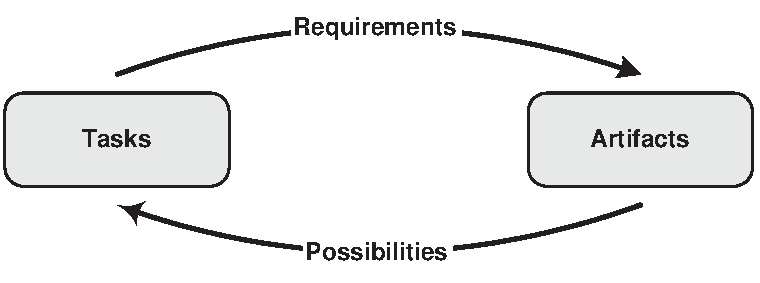
\includegraphics[height=4cm]
		{pictures/research_review/Ch2-TaskArtefactCycle.pdf}
	\end{center}
	\caption{The Task-artefact Cycle~\citep{Carroll-cycle:91}}
	\label{fig:TaskArtefactCycle}
\end{figure}
%% see~\citep{jc-cycle:91, jc-cycle:92}

%%%%%%%%%%%%%%%%%%%%%%%%%%%%%%%%%%%%%%%%%%%%%%%%%%%
%%%%%%%%%%%%%%%%%%%%%%%%%%%%%%%%%%%%%%%%%%%%%%%%%%
% \subsection{Technology and application domains within HCI}
%%%%%%%%%%%%%%%%%%%%%%%%%%%%%%%%%%%%%%%%%%%%%%%%%%
%%%%%%%%%%%%%%%%%%%%%%%%%%%%%%%%%%%%%%%%%%%%%%%%%%%
%% Firstly personal information management is identified as an important application domain within HCI.%%
%%  Huge Area. Need to focus within HCI: use of application domains?
%% Sutcliffe's taxonomy of interface technologies and application domains~\citep{sutcliffe:00}:
%% \textit{Applications} (CHECK) e.g. personal information management, design genres? (abstractions over artifacts)
% Interactive systems exist in many forms. 
\citet{Sutcliffe:00} sets out a framework which can be used to classify HCI knowledge in terms of the forms of interactive system to which that knowledge applies. Sutcliffe classifies interactive systems in terms of  \textit{architecture families} and \textit{application/functionality families}.
Architecture families represent different types of user interface components such as speech recognition and window management.
Application families represent the task domains to which interface components can be applied. Examples include finance and information retrieval.

% Specific architectural components can be applied to a range of application areas. For instance speech recognition functionality can be applied to financial or information retrieval interfaces.
\textbf{Section~\ref{bg:pim}} defined PIM in terms of four user activities, the \textit{acquisition} of items to form a collection of information, the \textit{organization} of those items, the \textit{maintenance} of the collection, and the subsequent \textit{retrieval} of items to satisfy the user's information needs.  Therefore, within Sutcliffe's framework, PIM is an application family, to which interface technology can be applied.








% \newpage
%%%%%%%%%%%%%%%%%%%%%%%%%%%%%%%%%%%%%%%%%%%%%%%%%%%%%%%%%%%%%%%%%%%%%%%
%%%%%%%%%%%%%%%%%%%%%%%%%%%%%%%%%%%%%%%%%%%%%%%%%%%%%%%%%%%%%%%%%%%%%%%
\subsection{Research on Personal Information Management}
\label{review:pim-research-overview}
%%%%%%%%%%%%%%%%%%%%%%%%%%%%%%%%%%%%%%%%%%%%%%%%%%%%%%%%%%%%%%%%%%%%%%%
%%%%%%%%%%%%%%%%%%%%%%%%%%%%%%%%%%%%%%%%%%%%%%%%%%%%%%%%%%%%%%%%%%%%%%%
%% \textit{THINK: Use of task-artifact cycle as a framework for describing the area and the theory-practice gap?}
% THINK: relate studies -> design -> theory (with T/A cycle?
%%%%%%%%%%%%%%%%%%%%%%%%%%%%%%%%%%%%%%%%%%%%%%%%%%%%%%%%%%%%%%%%%%%%%%%
% ALternate structure:
% Frame as intra-tool/cross-tool from the start
%In terms of improving support - three fundamental research/design approaches can be identified:
%1.	RESEARCH: model as separate PIM systems with own distinct issues, DESIGN: Improve the interface of specific tools (i.e. optimize separately)
%2.	RESEARCH: investigate how tools are inter-linked, DESIGN: Improve integration between PIM tools (i.e. optimize inter-working) - yet retain separation/specialization where it makes sense
%3.	RESEARCH: model as one PIM system encompassing multiple applications, DESIGN: Unify PIM support.
%Many examples of all three types. Do we focus on one type here in survey?
%%%%%%%%%%%%%%%%%%%%%%%%%%%%%%%%%%%%%%%%%%%%%%%%%%%%%%%%%%%%%%%%%%%%%%%
\citet{Whittaker-rta:00} note the importance of everyday computer-based activities such as PIM.  They highlight three criteria of task importance: (1) tasks that are carried out frequently, (2) tasks that are ``mission-critical'', and (3) real-world tasks that are rooted in studies of actual user practice.  The studies of PIM discussed in the next section show how 
PIM matches the first and third of these criteria, confirming the promise of research in this area.  Since PIM-tools are in continual use by many millions of users, even small improvements to tool design may have profound effects in terms of productivity savings and satisfaction improvements.
% They discuss how PIM matches the first and third of these criteria.  The promise of research in this area can be framed as follows.
% Therefore there is a high worth in improving interface support for them)
% Many studies have noted the fundamental nature of personal information management -- it is carried out by millions of computer users  many times a day.

%%%%%%%%%%%%%%%%%%%%%%%%%%%%%%%%%%%%%%%%%%%%
% WHY RESEARCH IS WORTHWHILE IN THIS AREA
%%%%%%%%%%%%%%%%%%%%%%%%%%%%%%%%%%%%%%%%%%%%
%% Effect of increased IT support on productivity~\citep{landauer:95,sellen:01}

%% Quick overview of the main types/areas/strands/threads of research to explain structure of literature review see \textbf{Figure ~\ref{fig:chapter2_substantive_summary}}:
In this chapter three main areas of research related to PIM are discussed.
%%: (1) empirical studies, and (2) prototype design. 
%%%%%%%%%%
% STUDIES
%%%%%%%%%%
\begin{itemize}

\item \textbf{Section~\ref{review:pim-empirical-review}} reviews \textit{empirical studies of PIM behaviour}. This body of work has been concerned with understanding the usage of existing PIM artefacts, observing users' needs and problems, and making recommendations for improving design.
%% Empirical studies (trying to understand the activity of PIM by analysing the usage of existing PIM artefacts, observing users' needs and problems, and making recommendations for improving design)
%%%%%%%%%%
% DESIGN
%%%%%%%%%%

\item  \textbf{Section~\ref{review:pim-technological-review}} reviews \textit{technological prototyping}, the second body of research.  The design of research prototypes (the design of new artefacts aimed at providing improved support for user needs). The contribution of technology design to HCI knowledge is also considered.
%% Designing research prototypes (the design of new artefacts aimed at providing improved support for user needs). The contribution of technology design to HCI knowledge is considered in terms of artefact theory

%%%%%%%%%%
% THEORY
%%%%%%%%%%
% \textbf{Section~\ref{review:pim-theory-review}} reviews relevant theory.
\item \textbf{Section~\ref{review:pim-theory-review}} then discusses \textit{theoretical work relevant to PIM}. The overall lack of theory in this area is highlighted. Relevant theory from related fields such as information retrieval is also identified.

\end{itemize}



%%%%%%%%%%%%%%%
% SIGNPOSTING
%%%%%%%%%%%%%%%
% In the next three sections each area of research is considered, including the main methods employed and key contributions  made.  


%%%%%%%%%%%%%%%%%%%%%%%%%%%%%%%%%%%
%%%%%%%%%%%%%%%%%%%%%%%%%%%%%%%%%%%
%%%%%%%%%%%%%%%%%%%%%%%%%%%%%%%%%%%
%%%%%%%%%%%%%%%%%%%%%%%%%%%%%%%%%%%


\newpage
%%%%%%%%%%%%%%%%%%%%%%%%%%%%%%%%%%%%%%%%%%%
%%%%%%%%%%%%%%%%%%%%%%%%%%%%%%%%%%%%%%%%%%%
\section{Review of Empirical Work}
\label{review:pim-empirical-review}
%%%%%%%%%%%%%%%%%%%%%%%%%%%%%%%%%%%%%%%%%%%
% Studies to add:
% Dix (HCI-International): when best to file?
%%%%%%%%%%%%%%%%%%%%%%%%%%%%%%%%%%%%%%%%%%%
%%%%%%%%%%%%%%%%%%%%%%%%%%%%%%%%%%%%%%%%%%%%%%%%%%%%%%%%%%%%%%%%%%%%%
% Wording:
% 	a number of studies have examined / provide evidence that
%%%%%%%%%%%%%%%%%%%%%%%%%%%%%%%%%%%%%%%%%%%%%%%%%%%%%%%%%%%%%%%%%%%%%
%%%%%%%%%%%%%%%%%%%%%%%%%%%%%%%%%%
% Where to place?
% QUESTION: do results hold across multiple tools?
%%%%%%%%%%%%%%%%%%%%%%%%%%%%%%%%%%
% Generic vs. Task-Specific~\citep{bn-slides:96}
%%%%%%%%%%%%%%%%%%%%%%%%%%%%%%%%%


%%%%%%%%%%%%%%%
% SIGNPOSTING
%%%%%%%%%%%%%%%
% \textbf{Section~\ref{review:pim-research-overview}} identified the main bodies of research that are concerned with personal information management.
%%%%%%%%%%%%%%%%%%%%%%%%%%%%%%%%%%%%%%%%%%%%%
%% 2 types: lab studies and field studies
%%%%%%%%%%%%%%%%%%%%%%%%%%%%%%%%%%%%%%%%%%%%%
%% Fieldwork: chance to view evolution of stratgies
%% Lab-studies: non-interactive pre-specified tasks, pre-specified tasks, easy-to-define objective metrics, efficiency bias
%% Relative predominance of fieldwork compared to lab studies.  Postulate reasons why in pros and cons.
%%
%% Also varying levels of abstraction across workspace -- PIM-related problems can be tackled at many different levels.
%% although still far from a systematic background of knowledge~\citep{Whittaker-rta:00}. 
% The aim of empirical work is to investigate a phenomena  with the intention of  providing increased understanding of that phenomena in the form of empirical data or theory development.
% The aim of such work is to examine how users employ current tools, identify the problems they encounter, and are useful in highlighting the aspects of current tool designs that are non-optimal. 
% Within HCI, empirical studies have constituted a large proportion of research into PIM.
This section reviews the first body of research related to PIM, \textit{empirical studies}. 
The aim of such work has been to investigate the use of current PIM-tools, and to improve understanding of user behaviour and needs. The output of such research thus provides requirements for the design of new PIM-tools.
%%%%%%%%%%%%%%%%%%
% FIELD STUDIES
%%%%%%%%%%%%%%%%%%
% The downside is that users select their own tasks to some extent, and it may hard to compare between users~\citep{newman:95}. % Whittaker \textit{et al}.~\citep{Whittaker-rta:00} note the need to employ both objective lab studies and field studies in the investigation of personal information management and evaluating tools.
Two types of empirical work can be identified: (1) field studies, and (2) controlled studies.
Field studies follow in the ethnomethodological research tradition of collecting data in real-world, naturalistic contexts. In contrast, controlled studies emphasise the collection of objective data in a lab context. They typically involve the user in carrying out a pre-specified task, thus enabling comparison across multiple participants, rather than necessarily reflecting real-world usage. 

%%%%%%%%%%%%%%%%%%%%%%%%%%%%%%%%%%%%%%%%%%%%%%
%% Aim of empirical work
%%%%%%%%%%%%%%%%%%%%%%%%%%%%%%%%%%%%%%%%%%%%%%%
%% should really cite this
%% \textit{THINK: What is the aim of such empirical findings -- motivate and direct design? What are their inherent limitations?}
%%
%% Aim: raise issues, build up rich picture of how users employ tools, problems they encounter, identify particular needs and scope for new design
The rest of this section is structured as follows.  Firstly, \textbf{Section~\ref{field-studies}} moves on to consider field studies of PIM in both the physical and digital domains. Then \textbf{Section~\ref{objective-studies}} considers objective studies of low-level cognitive phenomena associated with PIM. Finally, \textbf{Section~\ref{empirical-contribution-discussion}} discusses the overall contribution from research of this type.

%%%%%%%%%%%%%%%%%%%%%%%%%%%%%%%%%%%%%%%%%%%%%%%%%%%%%%%%%%
\subsection{Field Studies}
\label{field-studies}
%%%%%%%%%%%%%%%%%%%%%%%%%%%%%%%%%%%%%%%%%%%%%%%%%%%%%%%%%%
% think also include ContactMap study?
%% EXPAND THIS SECTION IN DETAIL? - is G and D a field study?
%%%%%%%%%%%%%%%%%%%%%%%%%%%%%%%%%%%%%%%%%%

% This section is divided into studies of PIM in the physical and digital domains.

%%%%%%%%%%%%%%%%%%%%%%%%%%%%%%%%%%%%%%%%%%%%%%
\subsubsection{Studies in the physical domain}
%%%%%%%%%%%%%%%%%%%%%%%%%%%%%%%%%%%%%%%%%%%%%%
%% EXPAND EXPAND EXPAND aka "`More detail to be included here."'
As noted in \textbf{Chapter~\ref{chapter:bg}}, physical metaphors such as the Desktop Metaphor and the folder hierarchy have greatly influenced the design of PIM-tools~\citep{smith:82}.  A number of researchers have studied information management practices in the physical domain with the aim of influencing the design of digital PIM-tools.

%%%%%%%%%%%
% MALONE
%%%%%%%%%%%
% information management in the real world has provided a strong influence on the design of PIM-tools.  In particular, a number of  including the  have the standard form of PIM-tools is based on the desktop metaphor representation of physical offices.
% soper:76,cole:82,
% An early and influential body of empirical studies focused on the management of documents in offices, e.g. ,kwas:91}.  
Tom Malone's work has been particularly influential in PIM research~\citep{tm:83}.  Malone highlighted the inherent difficulties that many users encounter in classifying and retrieving documents in the physical domain, and identified a number of routes which PIM-tools could follow to avoid such problems in the digital domains.  These included support for automatic classification.  Malone also observed the fundamental \textit{reminding} affordance of desks -- people do not only arrange documents to find them again, they also do so to remind themselves of things to do (i.e. to contextualize their work activity).  By doing so, Malone went beyond the traditional information management perspective that focuses on storing items for future retrieval.  Malone also identified two fundamental user strategies in managing paper documents: \textit{filing} and \textit{piling}.
%%%%%%%%%%%
% KWASNIK
%%%%%%%%%%%
%In her study of physical PIM, Kwasnik~\citep{kwas:91}
%identified a range of factors that influenced the
%classification included those based on attributes of the
%document content such as author and topic, and those based
%on document context such as importance and activity. A
%similar technique has been employed more recently in the
%electronic domain in studies of applied similar methods to
%the electronic domain, in their studies of
%files~\citep{barreau:95} and web bookmarks~\citep{gd:01}.
%In contrast to these previous studies, the analysis
%presented here is based on folder names (and the
%descriptions participants offered of those folder names
%offered during the guided tour), rather than on
%participants' descriptions of their classificatory
%behaviour.
% More detail to be included here.
\citet{kwas:91} reports an investigation of classification practices in a physical office. Her study identified a number of contextual factors that influence classification decisions.  She concluded that people do not make classificatory decisions based purely on document attributes, e.g. title and author.  More recently, similar studies have been performed of the classification of files~\citep{barreau:95} and web bookmarks~\citep{gd:01}.
% Both of these studies have had a substantial influence on many later studies in the digital domain.

%%%%%%%%%%%%%%%%%
% More recent
%%%%%%%%%%%%%%%%
There have also been a number of contemporary studies in this area.  \citet{Whittaker-paper:01} took advantage of an office relocation to observe physical information management strategies. They present three main findings. Firstly, they observed that many people are irrational in terms of the information they manage, for instance they keep many items available elsewhere.  Secondly, they noted that many people employ a mixture of the piling and filing strategies identified by~\citet{tm:83}, and observed that filers tended to amass more information than pilers.  They also noted the importance of older archived information for many people, adding to the debate in this area (see next section). % ~\citep{bn:95,kidd:94,Gelernter:96a}.
%% define filers and pilers
\citet{sellen:01} note the large amount of time wasted by office managers in managing information, leading to a distraction from their primary job roles.  They suggest that there is a significant impact on manager productivity from PIM in the physical and digital domains.
%  More detail to be included here.
%% EXPAND EXPAND EXPAND aka "`More detail to be included here."'


%%%%%%%%%%%%%%%%%%%%%%%%%%%%%%%%%%%%%%%%%%%%%%%%%%%%%%%%%%
\subsubsection{Studies in the digital domain}
\label{digital-studies}
%%%%%%%%%%%%%%%%%%%%%%%%%%%%%%%%%%%%%%%%%%%%%%%%%%%%%%%%%%

Most studies in the digital domain have focused on user behaviour within specific PIM-tools.  This section highlights a number of key findings of relevance to the work in later chapters.  \textbf{Table~\ref{table:empirical_studies_summary}} offers a summary of the studies that have been performed.
%% More recent studies in the digital domain have focused on the various applications that support PIM.
The main focus to date has been on \textit{email}, e.g.~\citep{Whittaker-email:96,Ducheneaut:01}, \textit{web bookmarks}, e.g.~\citep{da:98,gd:01,kftf:01} and \textit{files}, e.g.~\citep{barreau:95,bn:95}.  In addition, many other types of personal information have been studied including \textit{photos}~\citep{kr:03}, \textit{time and task management}~\citep{sp:93,bg:01,palen:98}, \textit{contacts}~\citep{Whittaker-contacts:02}, \textit{instant messaging}~\citep{Whittaker-im:02}, and \textit{voicemail}~\citep{Whittaker-jotmail:00}.  Since the first three -- files, email and bookmarks -- act as the main focus of the empirical and design work in \textbf{Chapters~\ref{chapter:exploratory_study}} to \textbf{\ref{chapter:main-study}} of this thesis, they are also the focus of this review.  
%% 
% In general there is too much to survey, but some findings can be extracted that have relevance across multiple technological formats.


%%%%%%%%%%%%%%%%%%%%%%%%%%%%%%%%%%%%%%%%%%%%%%%%%%%%%%%
% TABLE: SUMMARY OF EMPIRICAL STUDIES
% Table generated by Excel2LaTeX from sheet 'Sheet1'
% in tables/ch2/ch2-tables.xls
%%%%%%%%%%%%%%%%%%%%%%%%%%%%%%%%%%%%%%%%%%%%%%%%%%%%%%%
\begin{small}
\begin{table}[hbtp]
\begin{center}
\begin{footnotesize}
\setlength{\extrarowheight}{2pt}
\begin{tabular}{|p{4cm}|p{7cm}|}
\hline
{\bf Type of information} & {\bf Studies} \\
\hline
Physical documents & \citep{tm:83,kwas:91} \\
\hline
Files (including the file system and desktop icons) & \citep{jc:82,akin:87,barreau:95,bn:95,Kaptelinin:96} \\
\hline
     Email & \citep{wm:88,Whittaker-email:96,ob:97,Ducheneaut:01} \\
\hline
Web bookmarks & \citep{da:98,gd:01,kftf:01,dix:03a} \\
\hline
    Images & \citep{kr:03} \\
\hline
 Voicemail & \citep{Whittaker-jotmail:00} \\
\hline
  Contacts & \citep{Whittaker-contacts:02} \\
\hline
Calendar and to-do items & \citep{sp:93,bg:01,palen:98} \\
\hline
Instant messaging & \citep{Whittaker-im:02} \\
\hline
\end{tabular}  

\end{footnotesize}
\caption{Summary of empirical studies of different PIM-tools}
\label{table:empirical_studies_summary}
\end{center}
\end{table}
\end{small}

%%%%%%%%%%%%%%%%%%%
% EMAIL DISCUSSION
%%%%%%%%%%%%%%%%%%%
% Email: generally most popular - although many studies focus on its usage as a collaborative tool. Whittaker~\citep{Whittaker-email:96}, Balter~\citep{ob:97,ob:00}, Duchaneaut~\citep{Ducheneaut:01}, Mackay~\citep{wm:88}. Also CSCW2002 workshop.
%%%%%%%%%%%%%%%%%%%
% WEB BOOKMARKS
%%%%%%%%%%%%%%%%%%%
% Web bookmarks: Abrams~\citep{da:97,da:98}, KFTF~\citep{kftf:01}, G\&D~\citep{gd:01}, Dix~\citep{dix:03a}

%%%%%%%%%%%%%%%%%%%%%%%%%%%%
% BARREAU
%%%%%%%%%%%%%%%%%%%%%%%%%%%%
Based on her study of file management, Barreau presents a conceptual framework that conveys the complex, high-level nature of PIM~\citep{barreau:95}.  In summary, she identified five aspects of the functionality provided by PIM-systems: (1) \textit{acquisition} of items into a collection, (2) \textit{organization} of items, (3) \textit{maintenance} of the collection (e.g. archiving items into long-term storage), (4) \textit{retrieval} of items for reuse, and (5) \textit{output} of the information in an appropriate format  This framework is discussed in more detail in \textbf{Section~\ref{bg:pim}}.  Barreau highlights the idiosyncratic nature of PIM leading to a wide variety of strategies between individuals, and the consequent need for tool flexibility. Barreau also notes the \textit{satisficing} nature of PIM: the people in her study only tended to acquire information as it was required, and only maintained their information when they were forced to by circumstances such as running out of space.
% More detail to be included here.

%%%%%%%%%%%%%%%%%%%%%%%%%%%%
% PROBLEMS
%%%%%%%%%%%%%%%%%%%%%%%%%%%%
%% MOVE TO LIMITS OF HIERARCHY STUDY? limits of hierarchy
Many studies have highlighted the problems users encounter in PIM sub-activities such as organization and retrieval.   % Many studies have concluded by calling for improved ``intelligent'' support for classification but it is not clear whether this would benefit users. Indeed many users choose not to use personal classification schemes, and instead rely on implicit metadata and search mechanisms for finding information . When users do file, they typically exhibit satisficing behaviour and ``just do enough to get by~\cite{barreau:95}.  This leads to problems such as premature filing and failed folders.
% Many of the studies of real-world PIM have noted the large amount of effort that users often devote to filing information (e.g. Bellotti and Smith 2000). Several researchers identify a trade-off between the time investment of up-front organization, versus the costs of not being able to find items in subsequent retrieval (B�lter 2000, Whittaker and Hirschberg 2001).
Lansdale highlights the core psychological difficulties inherent in the low-level processes of organization and retrieval~\citep{ml:88}.  He observes that classification is a cognitively difficult task with users having to deal with problems of ambiguous and overlapping categories. Users often employ a satisficing strategy, resulting in problems such as misfiling, failed folders, and filing prematurely before the value of an item has been assessed~\citep{Whittaker-email:96}.  Alternatively, users may not file, and rely on retrieving information via sorting based on implicit metadata, and search.  Such loose classification facilitates additional retrieval cues such as location, time and appearance. However, such strategies are rarely scalable (ibid).  Lansdale identifies two psychological processes that are used when retrieving information: (1) \textit{recall-directed search} (to home in on a group of items), and (2) \textit{recognition-based scanning} (selecting a particular item). He notes that retrieval systems are not tuned to the abilities of the human memory, such as  the ability to remember general meanings better than specific details. Users are forced to remember specific filenames and locations, whilst human memory is better at handling contextual information such as time and colour.
% The following technological criticisms have also been levelled against the
% folder hierarchy. 

%%%%%%%%%%%%%%%%%%%%%%%%%%%%%%%%%%%
% Types of personal information
%%%%%%%%%%%%%%%%%%%%%%%%%%%%%%%%%%%
%Several other researchers have proposed a similar break-down.
%%%%%%%%%%%%%%
% Also Soper, Malone?
%%%%%%%%%%%%%%
Several studies have surveyed the types of information that are managed by users.
\citet{bn:95} identify three types of information in terms of their lifetime of use: \textit{ephemeral}, \textit{working}, and \textit{archived}.  Ephemeral information is valued in the short-term and includes to-do items and information for immediate use.  Working information is valued over a longer period and may be kept for the period of a particular project over several months.  Archived information is kept in the long-term but is not in day-to-day use. There has been some disagreement over which is the most important type of information to focus on with design work. \citet{bn:95} highlight the relative importance of ephemeral/working information (accessed via location-based finding) over archived material (and the use of search).  This view is echoed by \citet{kidd:94} who argues that too much design is focused on supporting the management of older archived information.  In contrast, other researchers have argued the importance of archived information~\citep{Gelernter:96b,Whittaker-paper:01}.

%%%%%%%%%%%%%%%%%%%%%%%%%%%%%%%%
% \subsubsection{PIM strategies}
%%%%%%%%%%%%%%%%%%%%%%%%%%%%%%%%

Influenced by Malone's work, several studies have attempted to classify management strategies in various PIM-tools, with a particular focus on how users organize items. \citet{Whittaker-email:96} observed 3 types of strategies for managing email: \textit{frequent filer}, \textit{spring cleaner} and \textit{no-filer}. \citet{ob:97} extends this classification by dividing the no-filer class into two further sub-classes: \textit{folderless cleaner} and \textit{folderless spring-cleaner} (depending on whether old items are deleted from the inbox on a daily basis). \citet{da:98} proposed a similar classification of bookmark management strategies: \textit{no-filer}, \textit{creation-time filer}, \textit{end-of-session filer}, and \textit{sporadic filer}. The author is not aware of any strategy classifications in files.
% Within Barreau's model these classifications correspond to the organizing sub-activity, but as many of the above researchers note, they have a strong influence on the type of retrieval strategies employed.
%% Although note link from org/maint to retrieval strategies (more folders -- more browsing)

%%%%%%%%%%%%%%%%%%%%%%%%%%
% BROWSE VERSUS SEARCH
%%%%%%%%%%%%%%%%%%%%%%%%%%
In terms of retrieval, \citet{bn:95} identify a strong preference for location-based finding over the use of search.  They define location-based finding as the browsing of information via the organizational structure developed by the user. Their results have been strongly criticised by \citet{Gelernter:96a} who note that infrequent use of search can be explained by the poor design of search functionality in most operating systems. \citet{Gelernter:96a} call for further study of the use of advanced search technology.  However, it can be observed that later studies, including the one reported in \textbf{Chapter~\ref{chapter:exploratory_study}}, reinforce Barreau and Nardi's observation of a preference for browsing over search\footnote{The \textit{Stuff I've Seen} system~\citep{Dumais:03a} offers a unified search interface across a range of PIM-tools. Dumais \textit{et al}'s evaluation results suggest that the improved search technology in their prototype lead participants to depend less on filing and browsing-based retrieval.}.


%%%%%%%%%%%%%%%%%%%%%%%%%%%%%%%%%%%%%%
% Cross-tool/issues of integration
%%%%%%%%%%%%%%%%%%%%%%%%%%%%%%%%%%%%%%
% although the empirical body of work has made many pertinent observations and recommendations, a key limitation can be observed findings have been fragmented along tool/application boundaries. Little guidance is provided for the developers of integration/unification technologies.
%% segmentation of research
%% Application-centricity of requirements (piecemeal) -- knock-on influence on later stages of design (and choice of embedding, unifying design strategies)
% However there has been little consideration of PIM as a cross-tool phenomenon (one that involves the use of multiple tools).  Do individuals employ similar strategies in email as they do in files? How are these tools used together? These questions need to be addressed to provide an empirical foundation for the many systems proposed to improve integration between PIM tools (see below).
%%%%%%%%%%%%%%%%%%%%%%%%%%%%%%%%%%%%%%%%%%%%%%%%%%%%%%%%%%%%%%%%%%%%%%%%%%%%
%% But rare. Later than mine~\citep{goncalves:03a}
% One of the few other observations is by~\citep{bn:98} who observe users in need for better data transfer/handling of structured information.
%%  CHECK, should this be moved up into the strategy section above???
% \textit{A range of studies have focused on the sub-activities that make up PIM. \citet{jc:82} carried out a detailed study of the strategies used to name files in an early version of DOS. A number of studies have focused on the organization sub-activity of PIM~\citep{kwas:91,barreau:95,gd:01}.}
% Self-focused field studies in which researchers everything have also been carried out ~\citep{bell:01,pwilson:01,dix:02}. Provide vision of the ultimate PIM-tool, but it is not clear whether these prophecies reflect actual user needs or just the researchers' ambitions.
%% darpa-lifelog:03}
%% Total Recall http://bourbon.usc.edu/iml/recall/
%%%%%%%%%%%%%%%%%%%%%%%%%%%%%%%%%%%%%%%%%%%%%%%%%%%%%%%%%%%%%%%%%%%%%%%%%%%%
The prime focus of this thesis is on improving \textit{integration} between PIM-tools. 
However, few studies have investigated user behaviour beyond a tool-specific context.  Exceptions are discussed as follows. \citet{Kaptelinin:96,Kaptelinin:03} observes that users often employ multiple PIM tools in support of their high-level activities, such as the Desktop, the file system, and email.  He notes the difficulties users encounter in performing key project tasks across tool boundaries, such as archiving.   He also observes the duplication of organizational schemes between digital and physical documents.
\citet{Bellotti:00} similarly note how the management of information related to a particular activity is distributed across a wide range of tools.  Furthermore, they note that information of a particular technological format is often compartmentalized between different PIM-tools, e.g. files or reminders.  Like Kaptelinin, Bellotti and Smith observe the duplication of filing systems between different PIM-tools. However, neither study reports a detailed investigation of the extent of such duplication.  Two other studies have noted how users perform task and time management across a wide range of PIM-tools and physical artefacts~\citep{bg:01,Bellotti:03}.  Similarly, \citet{kftf:01} note how users manage web references with a wide range of mechanisms including bookmarks, email, ad-hoc lists, and physical print-outs.  All these studies make calls for improved integration between different tools. 



%%%%%%%%%%%%%%%%%%%%%%%%%%%%%%%%%
\subsection{Controlled Studies}
\label{objective-studies}
%%%%%%%%%%%%%%%%%%%%%%%%%%%%%%%%%

% \textit{They have been used primarily with this area to investigate low-level aspects of PIM.}

%% ADD: Hierarchy stuff (e.g. Williges stuff)
%  Use of 3D -- Robertson, Cockburn. \textit{Move to evaluations?}
% The previous section discussed field studies of personal information management. Here lab studies are considered. Note that study-based evaluations of PIM-tools are discussed in \textbf{Section~\ref{review:pim-technological-review}}.
% % Since they are not directly relevant to the scope of the thesis, a brief summary is provided as follows.
As well as field studies of naturalistic PIM behaviour, a number of controlled studies have also been carried out in the area.  Since the research reported in this thesis employs a field-study methodology, only a brief overview of two controlled studies is provided.  A number of controlled studies have also been carried out to evaluate new PIM designs (see \textbf{Section~\ref{review:pim-technological-review}}).

%%%%%%%%%%%%%%%%%%%
% DUMAIS AND JONES
%%%%%%%%%%%%%%%%%%%
% A number of studies have focused on how users classify information. 
%$ report a comparison of spatial versus symbolic means of storage and retrieval. ADD.
\citet{Dumais:85} carried out a paper-based experiment designed to test the frequent assumption that spatial memory is more effective than symbolic memory.  Participants were asked to organize a series of items, using a combination of location-based (spatial) and name-based (symbolic) filing systems.  Over a series of retrieval tasks, spatial filing was seen to offer no benefit over symbolic filing.  Furthermore, retrieval speeds for location-only deteriorated significantly as more items were added.  Based on their findings, Dumais and Jones suggest that spatial management should not replace symbolic techniques, but instead act as an adjunct, much as in current desktop computers.

% \citet{ml:88} report comparisons of user performance in recall versus recognition tasks. ADD.
% how the time at which bookmarks are filed affects retrieval performance.  ADD.
\citet{dix:03a} report an investigation of how retrieval performance depends on the time at which bookmarks are organized.  Two conditions were compared: ``sorting during browsing'', and ``sorting after browsing''.  Based on performance in a series of questions that involved retrieval from the set of bookmarks, the ``sorting after browsing'' resulted in significantly faster recall.  However, the difference was not evident when users were tested a week later.  Dix and Marshall suggest that the initial result may be due to the close proximity of the sorting and post-test tasks.  

A key criticism that can be levelled at such controlled studies is that they lack ecological validity. Although a number of interesting results are presented, the relevance of the findings to real-world contexts can be questioned.  Dix and Marshall themselves highlight two limitations of the ecological validity of their experiments: (1) the bookmarks were pre-selected, and (2) in real-life users may use a combination of during and after-browsing sorting.  \citet{Whittaker-rta:00} call for the employment of both field and controlled studies in PIM research.


%%%%%%%%%%%%%%%%%%%%%%%%%%%%%%%%%%%%%%%%%%%%%%%%%%%%%%%%%%%%%%%%
\subsection{Discussion of Empirical Contributions}
\label{empirical-contribution-discussion}
%%%%%%%%%%%%%%%%%%%%%%%%%%%%%%%%%%%%%%%%%%%%%%%%%%%%%%%%%%%%%%%%
% The section has so far reported the main findings from empirical studies directed at understanding the activity of PIM by analysing the usage of existing PIM artefacts, observing users' needs and problems, and making recommendations for improving design. Here the contribution offered by empirical studies is discussed and recommendations are expressed regarding the direction of future empirical research.

%%%%%%%%%%%%%%%%%%%%%%%%%%%%%%%
% 1. OVERALL: UNDER-RESEARCHED
%%%%%%%%%%%%%%%%%%%%%%%%%%%%%%%
%% %The general limitations of studies thaht have been carried out include questions over their statistical significance. e.g. closed user groups Knowledge Workers~\citep{kidd:94}
%% We now  We need more powerful PIM interfaces. Research from 1995 *should* be ignored. Discuss (-;
%% THINK about use of empirical findings?
% Generally studies have been aimed at providing increased understanding, make design recommendations, offer requirements for design, build theory.
% In terms of future research, in general more empirical groundwork is required in terms of the conceptual groundwork required for research in this area such as defining a descriptive vocabulary~\citep{Whittaker-rta:00}.
Although many interesting findings have been presented, the author echoes the view of~\citet{Whittaker-rta:00}, that there is still a lack of systematic empirical investigation in this area.  They propose a simple criterion for this: \textit{are there at least two user studies in a given area?}  Although this can be considered to be a highly conservative requirement given the ubiquity and importance of PIM, they note that even this criterion is not met. They conclude that there is no accepted body of knowledge to build further research on, for example a consensus of people's tasks and problems, and appropriate metrics for evaluation. % The lack of understanding can also be illustrated by the general disagreement over key issues such as the importance of PIM-tool support for different types of information. % In summary, the field is in an immature state.  Another limitation identified by the author is that technology has moved on from some of the se
% Although one or two studies have explored the usage of most tools in common use, Whittaker \textit{et al}. note that there is still a core lack of understanding. 
% A key cause of this situation is the complexity and range of phenomena associated with PIM. 
Three further limitations are identified by the author as follows.

%%%%%%%%%%%%%%%%%%%
% 2 INTEGRATION
%%%%%%%%%%%%%%%%%%%
The expressed focus of this thesis is on PIM-integration, and as the next section discusses there has been much design interest in this area. % It has been shown that a user will often employ multiple PIM tools in support of their high-level activities~\citep{Kaptelinin:96}. 
% there has been little consideration of PIM as a cross-tool activity (one that involves the use of multiple tools). 
However, the majority of studies have been tool-specific and are concerned with the management of information of a particular technological format (e.g. files, email, bookmarks). In terms of the wider personal information environment this represents an inherently piecemeal approach. \textbf{Section~\ref{review:discussion}} discusses this limitation in more detail.

%%%%%%%%%%%%
% 3 LONGIT
%%%%%%%%%%%%
%% A second limitation is the lack of attention to how PIM strategies may change over time. 
Another issue that illustrates the need for more studies in this area is the lack of empirical  attention paid to longitudinal aspects of PIM, e.g. how PIM strategies may change over time~\citep{ml:92}.  Instead, most work to date has been based on short-term ``snapshots'' of user behaviour % Exceptions are discussed~\citep{ob:97}. More understanding of longitudinal issues relating to PIM is required. Do PIM strategies change over time, and if so how?


%%%%%%%%%%%%%%%%%%%%%%%
% 4. WRONG TYPE OF USER
%%%%%%%%%%%%%%%%%%%%%%%
Finally, it is observed that most studies have focused on small groups of technical users.  It can be argued that such samples are unrepresentative of the wider population of users, including non-technical ``home'' users.
%% can I think of any counter-examples?
% It is noted that many of these users in early studies did not have hard disks, let alone email.  
% Users are much much more sophisticated today and have lots more info in lots more forms.  
Furthermore, many of the most often cited studies were carried out almost a decade ago, e.g.~\citep{bn:95}. For example, Barreau~\citep{barreau:95} mentions a few users who stored information on floppies as they did not have hard drives. Although some results will be transferable to modern personal information environments, it is envisaged that user needs may have moved on from 1995. % In other words further investigation is required. At the very least research should be extended to cover other types of user. The lack of work directed at  is highly evident.


%%%%%%%%%%%%%%
% TRANSFER
%%%%%%%%%%%%%%
% Finally it is noted that empirical findings have not been effectively used by other areas of research. For example little theory has been built on empirical data~\citep{ob:97,ob:00}, and there are few examples of how empirical data has been effectively leveraged in design~\citep{Bellotti:00,Whittaker-contactmap:02b}. Overall there is a lack of systematic understanding of users activities, problems, and needs to guide design work.


%%%%%%%%%%%%%%%%%%%%%%%%%%%%%%%%%%%%%
% \subsubsection{Directions for future empirical research}
%%%%%%%%%%%%%%%%%%%%%%%%%%%%%%%%%%%%%%

%%%%%%%%%%%%%%%
% SIGNPOSTING
%%%%%%%%%%%%%%%
%This section reviewed the first research area identified in \textbf{Section~\ref{review:pim-research-overview}}: empirical studies of PIM.
The next section discusses the second area of research contributions: the design and prototyping of new PIM-tool software.

%%%%%%%%%%%%%%%%%%%%%%%%%%%%%%%%%%%
%%%%%%%%%%%%%%%%%%%%%%%%%%%%%%%%%%%
%%%%%%%%%%%%%%%%%%%%%%%%%%%%%%%%%%%
%%%%%%%%%%%%%%%%%%%%%%%%%%%%%%%%%%%

\newpage
%%%%%%%%%%%%%%%%%%%%%%%%%%%%%%%%%%
%%%%%%%%%%%%%%%%%%%%%%%%%%%%%%%%%%
\section{Review of Technological Prototypes}
\label{review:pim-technological-review}
%%%%%%%%%%%%%%%%%%%%%%%%%%%%%%%%%%
% Possible alternative structures for this section.
% A) Divide as intra-tool, integrating, cross-tool.
% B) Use \textbf{Chapter 2} conceptual framework to structure design work
%		 (in terms of aspects of PIM, or technological formats).
% C) Divide as commercial, research-oriented
%%%%%%%%%%%%%%%%%%%%%%%%%%%%%%%%%%
%%%%%%%%%%%%%%%%%
% WHERE TO PLACE:
%%%%%%%%%%%%%%%%%
% \begin{itemize}
%	\item \textit{PIM Managers~\citep{kaplan:90}}
% \end{itemize}

%%%%%%%%%%%%%%%
% SIGNPOSTING
%%%%%%%%%%%%%%%
% \textbf{Section~\ref{review:pim-research-overview}} identified three main areas of research that have been concerned with personal information management.
% For the purposes of this literature review they are bundled with research-derived design.  
% current tools in the public domain and surveyed in .
%% Provide sign posting to traditional tool analysis/survey earlier in \textbf{Chapter~\ref{chapter:bg}} for survey of current commercial tools (see above).
\textbf{Section~\ref{bg:pim-tools}} surveyed PIM-tools in common use.  This section reviews exploratory PIM prototypes that have been proposed in the research domain, as well as highly innovative commercial systems that are not in widespread use.
%%%%%%%%%%%
% CAVEAT
%%%%%%%%%%%
% Since a wide range of work falls under this category, and the main concern in this thesis is to survey work aimed at providing integration between PIM-tools, only a representative summary is provided. A focus is taken on systems which have provided improved support for organization.
%% Both in research and commercial sectors.
This is an active area of design, and many systems have been proposed, particularly in the commercial sector. Therefore, this section does not aim to be an exhaustive summary, but to instead provide a representative summary.

%%%%%%%%%%%%%
% STRUCTURE
%%%%%%%%%%%%%
% A focus is taken on systems that aim to improve integration between PIM-tools.Three main design genres can be identified in terms of : (1) intra-tool design, (2) inter-tool integration, and (3) unification.
The section is structured in terms of four design genres, defined in terms of the \textit{level of integration} they provide:

\begin{itemize}

%%%%%%%%%%%%%%%%%%%%%%%%
% Tool-specific design
%%%%%%%%%%%%%%%%%%%%%%%%
%% Refer to web survey online?
%% \textit{THINK: Inherently out-of-date after publication!}
% The first genre is design aimed at improving support for the management of a particular type of information within an existing PIM tool - i.e. the optimization of independent PIM systems -- integration is not a main design aim. See  for an overview , but note this is not the main focus of the thesis.
\item \textit{Tool-specific design} -- \textbf{Section~\ref{review:intra-tool}} provides an overview of new technology aimed to improve the design of specific PIM-tools such as email.  Integration is not a primary design aim of such work.

%%%%%%%%%%%%%%%%%%%%%%%%
% Integration increase
%%%%%%%%%%%%%%%%%%%%%%%%
 % The second design genre is aimed at  -  See 
%% (e.g. Apple Data Detectors, the Context toolkit)
\item \textit{Systems that provide increased integration between distinct PIM-tools} -- \textbf{Section~\ref{review:integration}} surveys this second genre, aimed at improving integration between distinct PIM tools. %, i.e. retaining distinct PIM systems but providing  bridge between them.

%%%%%%%%%%
% EMBEDDING
%%%%%%%%%%
\item \textit{Designs that embed additional support for the management of multiple types of information within one PIM-tool} -- \textbf{Section~\ref{review:embedding}} covers the embedding design genre. % , which has focused on 

%%%%%%%%%%
% UNIFYING
%%%%%%%%%%
\item \textit{Unifying designs that consolidate the management of multiple types of information within a single interface} -- \textbf{Section~\ref{review:unifying}} covers this final genre which represents the most ambitious design work in this area.  % Within this genre two sub-genres can be identified: (1) \textit{embedding} designs, and (2) \textit{unifying} designs. 

\end{itemize}

% %%%%%%%%%%%%%%%%%%%%%%%%%%%%%%%%%
% FIGURE - PIM-tool design space
%%%%%%%%%%%%%%%%%%%%%%%%%%%%%%%%%%%
% \begin{figure}
%	\begin{center}
%		\leavevmode
%		
\includegraphics[height=2in, width=.9 \textwidth]{pictures/research_review/Ch2-TechDesignSpace.pdf}
%	\end{center}
%	\caption{PIM-tool design space}
%	\label{fig:review:tech_design_space}
%\end{figure}


%%%%%%%%%%%%%%%%%%%%%%%%%%%%%%%%%%%%%%%%%%%%%%%%%%%%%%%%%%%
\subsection{Intra-tool Designs}
\label{review:intra-tool}
%% expand on piles
%%%%%%%%%%%%%%%%%%%%%%%%%%%%%%%%%%%%%%%%%%%%%%%%%%%%%%%%%%%

This section considers design work within \textit{tool-specific} contexts.  Since the focus of the thesis is on the provision of improved integration between PIM-tools, only a representative sample of tool-specific work is provided.
% aimed at improving support for the management of specific types of information. This design genre is not concerned with improving integration between different technological formats. Instead the work described here is aimed at optimizing distinct PIM systems dedicated to managing information in a particular technological format.  Three areas of design are discussed.
% The main concern of this thesis is providing integration between PIM-tools, only a representative summary is provided. A focus is taken on systems which have provided improved support for organization.
%% Both in research and commercial sectors.


%%%%%%%%%%%%%%%%%%%%%%%
% automatic filing
%%%%%%%%%%%%%%%%%%%%%%%
% However, questions remain after their evaluation, notably the potential loss of control by the user.  In addition, 
%% EXPAND EVALUATION
Many studies have observed the problems encountered by users in classifying items, e.g.~\citep{tm:83,Whittaker-email:96}.  Several prototypes have offered automatic filing of email messages based on user modelling techniques, e.g. the \textit{Mailcat} system~\citep{mailcat:99}.  The system automatically processes incoming mail through an adaptive classifier, and suggests the three most likely folders for the message to be filed in.  A long-term study in the context of the authors' own email usage revealed an accuracy rate of 85\%.  Although later systems have improved performance, such systems require some level of user monitoring which may be problematic.  Furthermore, \citet{Shneiderman:97} observe that such intelligent interfaces may result in a loss of control on the part of the user.


%%%%%%%%%%%%%%%%%%%%%%%%%%%%%
% multiple classification
%%%%%%%%%%%%%%%%%%%%%%%%%%%%%
% Aim here to deal with limitations of file+folder paradigm within the context of a specific type of information. 
% \textit{Haystack} system is set apart by the fact that a published evaluation has been performed. The evaluation was performed within the context of a controlled study.  Although the system was received positively, no objective improvements in retrieval time were observed. The need for a follow-up long-term evaluation is highlighted in the context of users's natural behaviour and information. %  Furthermore, the evaluation task was not a natural example of bookmark management which happens incrementally over time for many users~\citep{da:98}. 
Other prototypes have focused on a key limitation of the folder hierarchy, that of multiple classification not being supported, e.g.~\citep{haystack:03b}. Several commercial tools also provide multiple-classification support including \textit{BookKey} and \textit{GMail}.    Such systems allow a user to assign arbitrary user-defined attributes to an item, and then to retrieve them using any combination of those attributes.  Quan \textit{et al} report an evaluation of a multiple classification interface for managing bookmarks based on a flat set of attributes.  Users welcomed the multiple classification functionality, and there was some improvement in retrieval speed. However, the experiment can be criticized in terms of ecological validity, as a pre-selected data set was employed.  Furthermore, several limitations were observed including: (1) duplicated attributes, and (2) poor support for data that is naturally hierarchical.  The author urges further evaluation in a real-world setting.


%%%%%%%%%%%%%
% PILES
%%%%%%%%%%%%%
% At the small scale: piles~\citep{piles:92}. More detail to be included here.
%% think should piles be in spatial area?
%% EXPAND EXPAND EXPAND aka "`More detail to be included here."'


%%%%%%%%%%%%%%%%%%%%%%%%
% visualization schemes
%%%%%%%%%%%%%%%%%%%%%%%%%
% allowing the user to perform  by leaving items in piles
% A number of other prototypes have provided improved support for the visualization of hierarchical information (e.g. treemap, polyarchy work at Microsoft).
% On the desktop, the Piles system replicates piles of documents observed in the physical context~\citep{tm:83} in a digital context, and thus facilitates 
Other tool-specific work has offered new interactive techniques for representing collections of items.  The \textit{Piles} system~\citep{piles:92} allows the ``casual organization'' of items, a digital equivalent to the piling strategies observed by Malone in physical office environments~\citep{tm:83}. 
%%%%%%%%%%%%%%%%%%%%%%%%%%%%%%%%%%%%%%%%%%%%%%%%%%%%%%%
% \subsubsection{Spatial approaches to unification}
%%%%%%%%%%%%%%%%%%%%%%%%%%%%%%%%%%%%%%%%%%%%%%%%%%%%%%%
% RECONSIDER: is spatial really means of unification?
%%%%%%%%%%%%%%%%%%%%%%%%%%%%%%%%%%%%%%%%%%%%%%%%%%%%%%%
% A number of systems have been proposed that allow multiple types of personal information to be managed spatially. Three main types can be identified. The first type are spatial systems such as ROOMS~\citep{rooms:86} and Task Gallery~\citep{gr:00} which are more an integrative framework within which applications can exist. These can be considered alternatives or extensions of the desktop metaphor.
% More detail to be included here.
% Also consider Info Viz~\citep{card:91,card:96}
%% EXPAND EXPAND EXPAND aka "`More detail to be included here."'
% Second, there systems that provide spatial 
% More detail to be included here.
%% EXPAND EXPAND EXPAND aka "`More detail to be included here."'
%The final type are spatial hypertext systems~\citep{shipman:01}.
% More detail to be included here.
% Question: has this been evaluated? Is PIM a main design aim of this?
%% EXPAND EXPAND EXPAND aka "`More detail to be included here."'
Other prototyping has offered 3D spatial environments for managing information such as bookmarks, e.g. \textit{Data Mountain}~\citep{gr:98}.  However, the benefits of such a 3D approach have been questioned in follow-up work~\citep{ac:01}. Although users preferred the 3D interface, Cockburn and McKenzie observed slower retrieval times compared to a 2D system.

%% or email stuff from Lotus. TIDY

%%%%%%%%%%%%%%%%%%%%%%%%%%%%%%%%%%%%%%%%%%%%%%%%%%%%%%%%%%%%%%%%%%%%%%
% Other examples of intra-tool design that can be left out for now
%%%%%%%%%%%%%%%%%%%%%%%%%%%%%%%%%%%%%%%%%%%%%%%%%%%%%%%%%%%%%%%%%%%%%%
%Other prototypes have been poroposed to provide mproved support for specific technological formats including images~\citep{kuch:99,kr:03}, bookmarks (Saul stuff, Hunter-Gatherer, YelloPen) and voicemail~\citep{Whittaker-jotmail:00,Whittaker-scanmail:02}.

%%%%%%%%%%%%%%%%%%%%%%%%%
%%%%%%%%%%%%%%%%%%%%%%%%%
%%%%%%%%%%%%%%%%%%%%%%%%%
%%%%%%%%%%%%%%%%%%%%%%%%%


%%%%%%%%%%%%%%%%%%%%%%%%%%%%%%%%%%%%%%%%%%%%%%%%%%%%%%
\subsection{Improving Integration between Distinct PIM-tools}
\label{review:integration}
%%%%%%%%%%%%%%%%%%%%%%%%%%%%%%%%%%%%%%%%%%%%%%%%%%%%%%
% In this section designs are described which retain the separation between tools that manage different types of information, but attempt to improve integration between them. % Systems which go the whole way are discussed in the next section. 
%%
% Note that 
%% \textit{THINK: (OVERLAP ABOVE with current technology). 
%% Many areas, consider using a ``workspace diagram'' to frame all the different integration-related problems}
% A number of research systems have provided new forms of integration between current, distinct PIM-tools. 



%%%%%%%%%%%%%%%%%%%%%%%%%%%%
% STRUCTURED INFORMATION
%%%%%%%%%%%%%%%%%%%%%%%%%%%%
% Structured information, such as web addresses and email addresses appears in a wide range of personal information. Such structured information follows a standard format and can be easily identified by straight-forward pattern matching software.
% Current PIM-tools provide integration with other PIM-tools by allowing the user to select structured information embedded in an item, to enable access to, or storage of that information in another PIM-tool.  For example Microsoft Outlook allows the user to select a web/email address within an email message and open it within a web browser. % Other tools allow the user to go further and add the web address directly into their bookmark collection.
% Integration between PIM-tools is provided by allowing access to information in one technological format from within a collection dedicated to a different technological format.
% \textit{Also transfer between collections that support different technological formats}.
Current PIM-tools, such as MS-Outlook, offer limited integration based on some kinds of structured information, e.g allowing the user to access the contact manager by selecting an email address in a message (see \textbf{Section~\ref{bg:integration}}). Two research systems have proposed more powerful integration based on structured information. 
%%%%%%%%%%%%%%%%%%%%%%%%%%
%% Apple Data Detectors
%%%%%%%%%%%%%%%%%%%%%%%%%%
% A scripting language is provided to allow the construction of grammars to match other forms of structured information, and the specification of other actions to execute.
The \textit{Apple Data Detectors} system~\citep{bn:98} parses a selected region of text for a range of structured information including dates, postal addresses, meeting information and phone numbers. For example, the recognition of a date within the selected region allows it to be placed within a calendar as a meeting, along with the surrounding text.  This technology should also be highlighted for two reasons: (1) it is rooted in study data highlighting a user need for taking action on structured information~\citep{bn:95}; and (2) the system is one of the few examples of PIM-related design research that has found its way into a commercial product -- Apple MacOS.
%%%%%%%%%%%%%
% Cyberdesk
%%%%%%%%%%%%%
% possible for users to subsequently define further integration based on other forms of structured information.
% Therefore, selecting an email address in a message 
% extensible processing of structured information, for example chaining functions in multiple tools, e.g.  allowing a web search based on a name, or the look-up of an email address associated with a name.
\citet{dey:98} highlight a key limitation of standard integration based on structured information: such integration must be pre-defined by the software developer. %, it is not 
They propose a system called \textit{Cyberdesk} which allows the user to define how different types of structured information should be processed.  Furthermore, the system enables the \textit{chaining} of processing across multiple tools.  However, Cyberdesk can be criticised for a lack of evaluation, and it is not clear if users require such advanced functionality. % both these tools can be criticised in terms of ease-of-use as rogramming skills are required for generating new grammars and integrating new applications. Additionally, evaluations have not been published.


%%%%%%%%%%%%%%%%%%%%%%%%%%%%%%%%%%%%%%%%%%%%%%%%%%%%%%%%%%%%%%%%%%
% \subsubsection{Search-based unification}
%%%%%%%%%%%%%%%%%%%%%%%%%%%%%%%%%%%%%%%%%%%%%%%%%%%%%%%%%%%%%%%%%%
% Other systems have provided unified access to multiple technological formats of personal information via a \textit{consolidated search mechanism}. % The principles of such content-based search is discussed in~\citep{norman:93}. Examples include \textit{Stuff-I've-Seen}~\citep{Dumais:03a,Dumais:03b} and \textit{MyLifeBits}~\citep{bell:02}. % Both are Microsoft Research projects with much the same functionality -- the ability to search multiple types of personal information with one query.
% �	Dumais et al. (SIGIR 2003), Stuff I've Seen - cross-tool search -based. Focuses on search/retrieval. EXPAND.
%%%%%%%
% SIS
%%%%%%%
The \textit{Stuff-I've-Seen (SIS)} system~\citep{Dumais:03a} offers search-based unification, giving users the ability to search multiple PIM-tools with one query\footnote{A number of commercial systems have also been proposed which offer equivalent functionality, e.g. SixDegrees. This is an add-on layer on top of existing applications that performs semantic clustering of related files, email and bookmarks related to a selected item.}.   The system builds a unified index of all personal information.  Result sets are provided in time-ordered sequence, annotated with thumbnails and item previews.  Dumais \textit{et al.} report a field-study based evaluation which revealed significant system up-take, and less frequent use of tool-specific search mechanisms.  Additionally, feedback from users suggested that they would be less likely to organize items in distinct folder hierarchies, if operating systems provided \textit{SIS}-like functionality.

% It is set apart from most other PIM-unification approaches by its evaluation. 


%%%%%%%%%%%%%%%%%%%%%%%%%%%%%%%%%%%%%%%%%%%%%%%%%%%%%%%%%%%%
% \subsubsection{Other forms of inter-tool integration}
%%%%%%%%%%%%%%%%%%%%%%%%%%%%%%%%%%%%%%%%%%%%%%%%%%%%%%%%%%%%
% Alternative title: Syanchronization and data-access technology}
%%%%%%%%%%%%%%%%%%%%%%%%%%%%%%%%%%%%%%%%%%%%%%%%%%%%%%%%%%%%
%%%%%%%%%%%%%%%%%%%%%%%%%%%%%%%%%%%%%%%%%%%%%%%%%%%%%%%%%%
%% THINK carefully about the placement of all this stuff
%%%%%%%%%%%%%%%%%%%%%%%%%%%%%%%%%%%%%%%%%%%%%%%%%%%%%%%%%%
% Synchronization facilitates a form of integration between collections of a particular technological format, typically on distinct computers.  Prototypes have been developed to provide more advanced synchronization between computers (e.g. ~\citep{roma:00})
%% think: why is this so exiciting?
%%%%%%%%%%%%%%%%%%
% REMOTE ACCESS
%%%%%%%%%%%%%%%%%%
% Related to synchronization, are ``remote access'' systems. Such systems allow remote access to one centralized store of information from multiple devices/places. Many commercial systems exist to offer such functionality including so-called identity management systems that allow people to store personal details for e-commerce applications. Such systems also facilitate the management of personal information such as files and email that can then be accessed from miscellaneous devices.  
%%%%%%%%%%%%%%%%%%%%%%%%%%%%%%%%%%%%%%%%%%%%%%%%%%%
%% but why is this any different to Yahoo! mail?
%%%%%%%%%%%%%%%%%%%%%%%%%%%%%%%%%%%%%%%%%%%%%%%%%%%
%% Information/remote access (e.g. Pocketwatch) COMMERCIAL.
% Example functionality includes providing a 
% raise  including the trust required on the part of users to entrust all their personal information to a third-party.
So-called ``identity management systems'', such as Microsoft .NET Services, provide server-side integration by offering a central repository for personal information such as email, contacts and folders, which can then be accessed from different PIM-tools on different devices.
However, such centralized systems require users to entrust personal information to a third-party, resulting in numerous privacy issues.

%%%%%%%%%%%%%%%%%%%%
% DIGITAL PHSYICAL
%%%%%%%%%%%%%%%%%%%%
As well as providing integration between PIM-tools in the digital domain, research has also focused on enabling integration between the digital and physical domains. The \textit{Protofoil} system~\citep{rao:94} allows the management of paper documents as electronic images, including the retrieval of paper documents via keyword search.
%% 
%% CONSIDER: Hypertext-based application integration?


%%%%%%%%%%%%%%%%%%%%%%%%%
% LINK
%%%%%%%%%%%%%%%%%%%%%%%%%
% % Two approaches are considered: (1) , and (2) unifying interaction with multiple types of information (e.g. files, email and bookmarks) within a consolidated interface.These are discussed in  and  respectively.
The next two sections consider systems that provide support for managing multiple types of information within a single interface. Firstly, \textbf{Section~\ref{review:embedding}} considers the embedding of support for managing non-native information formats within a PIM-tool.



%%%%%%%%%%%%%%%%%%%%%%%%%%%%%%%%%%%%%%%%%%%%%%%%%%%%%%
\subsection{Embedding Designs}
\label{review:embedding}
%%%%%%%%%%%%%%%%%%%%%%%%%%%%%%%%%%%%%%%%%%%%%%%%%%%%%%

% Common to all these approaches is that they provide integrating mechanisms between distinct collections of information. PIM-tools are treated as distinct PIM-systems with their own support for PIM sub-activities such as organization and maintenance. However the segmented management of different types of personal information is retained.
% This section deals with technological design that attempts to \textit{embed} support for multiple types of personal information (technological formats) within one interface
Current PIM tools focus on the management of information in a specific technological format. The main exceptions are the file system in which many technological formats can be stored, and email which allows the user to manage non-native items, such as files, as message attachments.  

% Current email clients enable the management of documents as attachments to email. In other words email is the primary technological format.
% This is defined as the tool's primary technological format. Thus embedding is defined as adding support for additional technological formats into a tool dedicated to a different primary format.
%% exception: PIM managers a la Agenda
A number of research systems allow the user to manage multiple types of information with one PIM-tool, through the \textit{embedding} of extra functionality. 
% Embedding is to be contrasted with unifying systems which are not based on a primary technological format -- but enable management of multiple types.
There has been a particular focus in the literature on embedding support for non-native information within email clients~\citep{Bellotti:00,Bellotti:03,Gwizdka:02}.  The prototypes developed by Bellotti \textit{et al}. allow the management of email, documents, and to-do items as ``first class citizens'' which can co-exist in the tool's main ``inbox''.  The main design rationale for the embedding approach is the observation that email acts as a ``habitat'' for a wide range of user activities~\citep{Bellotti:00,Ducheneaut:01}. This causes users to develop ad-hoc means of managing information such as to-dos within email.


% Empirical observations of email tools acting as a habitat fpr  for user activity act as .
%% CHECK AND ALSO MENTION EVALUATIONS CARRIED OUT
% �	Bellotti et al. (CHI 2003), TaskMaster - embedding PIM support in email. Evaluation over a series of weeks. Increases complexity of email. No consideration of how PIM in other tools affected. 
\citet{Bellotti:03} report the field-study evaluation of their \textit{TaskMaster} email client which as well as supporting the management of multiple types of information, also provides a mechanism for labelling any item of information with to-do metadata.  Bellotti \textit{et al.} note the challenges inherent in providing a sufficiently robust prototype to withstand long-term usage.  Despite these methodological issues, both sets of extra functionality were received positively by test users.  However, it is noted that the test users were technically experienced.  A key criticism of the embedding approach is that it increases the complexity of already complex tools, and therefore may not be suitable for less technical users. For example, the \textit{Raton-Laveur} prototype~\citep{Bellotti:00} includes no less than three organizing mechanisms.

% It can also be noted that many designs have been highly complex and aimed at expert users.
% ADD EVALUATION: PROMISING.  However,  
% In effect the email tool becomes the main workspace. However outside the email tool the familiar range of compartmentalized applications still exists. 
%% ADD MAIN RESULTS OF EVALUATION

%%%%%%%%%%%%%%%%%%%%%%%%%
%%%%%%%%%%%%%%%%%%%%%%%%%
%%%%%%%%%%%%%%%%%%%%%%%%%
%%%%%%%%%%%%%%%%%%%%%%%%%

%%%%%%%%%%%%%%%%%%%%%%%%%%%%%%%%%%%%%%
\subsection{Unifying Designs}
\label{review:unifying}
%%%%%%%%%%%%%%%%%%%%%%%%%%%%%%%%%%%%%%

This section surveys systems that unify the management of multiple types of information within a new consolidated interface, rather than embedding it within an existing tool.  Two types of unifying system can be identified:
\begin{itemize}

% \item Is the system based on a dominant organizational dimension such as role, project, person or time? Organizational dimension is defined as the type of concept used to organize items. For instance, a folder ``Bill'' is based on the organizational dimension of person.
\item Systems that unify the management of multiple types of information within an interface based on a dominant \textit{organizational dimension} such as role, project, or time.

% Does the system offer an alternative organizational paradigms to the traditional hierarchy? Many of the systems described in this section do offer alternatives to the file+folder metaphor.
\item Systems which do not enforce a particular organizational dimension.  Approaches include search-based, attribute-based and hypertext-based unification.
\end{itemize}

% Firstly systems based on a dominant organizational dimension are discussed.  
Firstly, systems based on a dominant organizational dimension are surveyed.  \textbf{Table~\ref{table:unification_dominant_orgdim}} provides an overview of this body of design work.  The following sub-sections discuss each organizational dimension in turn.
%%
% These systems can be classified along the following dimensions:
% \begin{enumerate}
% \item Does the system completely replace other PIM-tools? If not the system is effectively another parallel management interface.



%%%%%%%%%%%%%%%%%%%%%%%%%%%%%%%%%%%%%%%%%%%%%%%%%%%%%%%
% TABLE: UNIFICATION BASED ON SINGLE ORG DIM
% Table generated by Excel2LaTeX from sheet 'Sheet2'
% in tables/research_review
%%%%%%%%%%%%%%%%%%%%%%%%%%%%%%%%%%%%%%%%%%%%%%%%%%%%%%%
\begin{small}
\begin{table}[hbtp]
\begin{center}
\begin{footnotesize}
\setlength{\extrarowheight}{2pt}
% Table generated by Excel2LaTeX from sheet 'Unification - 1o org dimension'
\begin{tabular}{|p{4cm}|p{6.5cm}|c|}
\hline
{\bf Organizational Dimension} & {\bf System} & {\bf Evaluation} \\
\hline
Time & \textit{MEMOIRS}~\citep{ml:92}, \textit{Lifestreams}~\citep{Gelernter:96a} &     no \\
\hline
Role & \textit{Role Manager}~\citep{Shneiderman:94} &         no \\
\hline
Project & \textit{UMEA}~\citep{Kaptelinin:96} &   informal \\
\hline
Contact & ContactMap~\citep{Whittaker-contactmap:02b} &         no \\
\hline
\end{tabular}  
\end{footnotesize}
\caption{Unification designs based on a dominant organizational dimension}
\label{table:unification_dominant_orgdim}
\end{center}
\end{table}
\end{small}


%%%%%%%%%%%%%%%%%%%%%%%%%%%%%%%%%%%%%%%%%%%%%%%%%%%%%%%%%%%%%%%%%%
\subsubsection{Time-based Unification}
%%%%%%%%%%%%%%%%%%%%%%%%%%%%%%%%%%%%%%%%%%%%%%%%%%%%%%%%%%%%%%%%%%

A number of PIM-unification prototypes have been based on chronological organization of personal information. Three examples are discussed here: \textit{MEMOIRS}~\citep{ml:92}, \textit{LifeStreams}~\citep{Gelernter:96a}, and \textit{Milestones} system~\citep{Dumais:03b}.

%%%%%%%%%%%%%
% MEMOIRS
%%%%%%%%%%%%%
The \textit{MEMOIRS} system~\citep{ml:92} is founded on the principle of organizing all information in terms of \textit{events}. \textit{MEMOIRS} is based on the integration of the diary and filing system, with files managed in the same chronological mechanism as events such as meetings.  Although the implemented prototype did not cater for other types of personal information such as email, this extension was envisaged.
%%
The system was proposed as a vehicle to explore the application to design of findings from cognitive psychology.  The primary design aim was to enable retrieval based on temporal context, thus exploiting autobiographical memory.  A second was to promote retrieval by recognition (based on visual appearance) rather than recall. This was enabled by allowing items to be colour coded.  % related to autobiographical memory. A range of empirical findings were used to direct design such as higher accuracy of recognition over recall.
% Not a product but a design hypothesis: \textit{``at experiment aimed at addressing the question -- how far can user's memory for documents be exploited in the design of a filing system?''}.
%%%%%%%%%%%%%%%%%
% EVALUATION
%%%%%%%%%%%%%%%%%
Lansdale and Edmonds stress the importance of long-term evaluation, particularly when using  ``fundamental research'' such as cognitive psychology to direct high-level design.  They note that many such findings, may not apply in a natural setting.  Despite their concerns, \textit{MEMOIRS} has not been evaluated.

%%%%%%%%%%%%%%%
% LIFESTREAMS
%%%%%%%%%%%%%%%
Another notable time-based PIM-unification prototype is \textit{Lifestreams}~\citep{Gelernter:96a,Gelernter:96b} which provides a time-ordered organization of all personal information. The Lifestreams system has now been realised as a commercial tool called \textit{Scopeware}. Although the tool appears to have been received well based on press reports, the contribution in terms of HCI research is limited as no evaluation has been published.  Both MEMOIRS and LifeStreams combine a primary chronological organizational mechanism with attributed-based organization of items.  The attributed-based approach is detailed on page~\pageref{review:pim-technological-review:attribute}. %, as an alternative to the hierarchical file/folder paradigm.

%%%%%%%%%%%%%%%%
% MILESTONES
%%%%%%%%%%%%%%%%
A final example is the \textit{Milestones} system~\citep{Dumais:03b} which organizes cross-tool search results in a time-line visualization annotated with ``landmarks'' corresponding to a user's personal information such as events and images.  The reported evaluation suggests benefits from the landmarks in terms of retrieval time over a plain time-ordered result set.

%%%%%%%%%%%%%%%%%%%%%%%%%%%%%%%%%%%%%%%%%%%%%
%% CONSIDER ADDING TIME_MACHINE COMPUTING
%%%%%%%%%%%%%%%%%%%%%%%%%%%%%%%%%%%%%%%%%%%%%
% The ``Time machine computing'' prototype~\citep{rekimoto:99} allows spatial arrangements of personal information to be ``fast-forwarded'' and ``rewound'' in time. CONSIDER INCLUDING
%% \textit{Also see spatial approach (CONSIDER MOVE?)}
%
% ADD: Milestones/Landmarks system~\citep{Dumais:03a,Dumais:03b}.

%%%%%%%%%%%%%%%%%%%%%%%%%%%%%%%%%%%%%%%%%%%%%%%%%%%%%%%%%%%%%%%%%%
\subsubsection{Contact-based Unification}
%%%%%%%%%%%%%%%%%%%%%%%%%%%%%%%%%%%%%%%%%%%%%%%%%%%%%%%%%%%%%%%%%%
% The system is based on the dominant organizational dimension of person.
% The user interface is centred on a visual representation of the social network .
The \textit{ContactMap} system~\citep{Whittaker-contactmap:02b} integrates the management of multiple types of personal information based on the representation of a user's social network, 
derived from the user's address book.  The interface offers a spatial map of the social network and enables access to files, email and bookmarks associated with contacts, as well as to communication functionality for contacting that person. Awareness information is also provided. Thus ContactMap integrates both information management and communication functionality.
% This system is one of the few examples of PIM-unification prototypes that is grounded in empirical requirements. Nardi \textit{et al}. note the large extent to which many people rely on social networking information in carrying out their work.  However such contact information is typically limited to the contact manager software and low-level metadata associated with specific items.  They identify a range of activities which users currently encounter such as tracking documents associated with a particular contact. ContactMap is proposed to explore the worth of using a social network in a much more prominent position with in the workspace, as the dominant organizational paradigm.
Although Nardi \textit{et al}. carry out an empirical investigation into the generation of social networks from users' contact data, no evaluations of system usage have been published. % For instance it is not clear whether ContactMap would be taken up in place of traditional PIM-tools or would be used as an extra tool.
However, communication with one of the authors indicates that an evaluation is soon to be published~\citep{Whittaker-personal:03}.



%%%%%%%%%%%%%%%%%%%%%%%%%%%%%%%%%%%%%%%%%%%%%%%%%%%%%%%%%%%%%%%%%%
\subsubsection{Activity-based Unification}
%%%%%%%%%%%%%%%%%%%%%%%%%%%%%%%%%%%%%%%%%%%%%%%%%%%%%%%%%%%%%%%%%%

Two PIM-unification prototypes focus on a user's \textit{activities} as the dominant organizational dimension: \textit{Personal Role Manager}~\citep{Shneiderman:94} and \textit{UMEA}~\citep{Kaptelinin:96}.

%%%%%%%%%%%%%%%%%%%%%%%%%%%%
% ROLES: The Role Manager
%%%%%%%%%%%%%%%%%%%%%%%%%%%%
The \textit{Personal Role Manager}~\citep{Shneiderman:94} allows the user to manage multiple technological formats under the dominant organizational dimension of \textit{roles}, a user's high-level activities. Roles can in turn be broken down into a task hierarchy represented as windows in which relevant files can be stored.  The role and task descriptions are also made available in the user's calendar.
% User roles are defined as long-term user activities.
% More detail to be included here.
However, like many other PIM-unification systems, no evaluation has been reported.
%% EXPAND EXPAND EXPAND aka "`More detail to be included here."'

%%%%%%%%%%%%%%%%%%%%%%%%%%%%%%%%%%%%%%%%%%%%%%%%%%%%%%%%%%%%%%%%%%
% PROJECTS: UMEA
%\subsubsection{Project-based unification}
%%%%%%%%%%%%%%%%%%%%%%%%%%%%%%%%%%%%%%%%%%%%%%%%%%%%%%%%%%%%%%%%%%
The \textit{UMEA} system~\citep{Kaptelinin:96,Kaptelinin:03} allows the user to organize multiple types of information in terms of their high-level projects.  The design rationale is based on the observation that a user's activities often involve multiple PIM-tools.  The system allows a user to specify the current project which is being worked on.  Thereafter, all information that the user interacts with, is automatically associated with that project.
An informal evaluation was carried out, resulting in positive feedback from several users regarding the principle of project-centric unification.  However one limitation was the need for the user to switch task manually.  This is especially problematic in tool contexts where high-level activities are likely to be interleaved, e.g. email.  Kaptelinin acknowledges the need for a follow-up, in-depth evaluation. % This is clearly not an in-depth evaluation which limits the contribution offered by this system.
% �	Kaptelinin (CHI 2003), UMEA system - share project-based metadata cross tools. My design has a similar aim - allowing cross-tool organization (in his case, based on projects), but his evaluation very very sketchy. Theoretical motivation, not empirical.




%%%%%%%%%%%%%%%%%%%%%%%%%
%%%%%%%%%%%%%%%%%%%%%%%%%
%%%%%%%%%%%%%%%%%%%%%%%%%
%%%%%%%%%%%%%%%%%%%%%%%%%




%%%%%%%%%%%%%%%%%%%%%%%%%%%%%%%%%%%%%%%%%%%%%%%%%%%
\subsubsection{Attribute-based Unification}
\label{review:pim-technological-review:attribute}
%%%%%%%%%%%%%%%%%%%%%%%%%%%%%%%%%%%%%%%%%%%%%%%%%%%
% % Many of these consolidated interfaces have been based on alternatives to the file+folder paradigm. MIXED AIMS: It should be noted that improving integration between PIM-tools is only one of the design aims of many of these tools. Another primary design aim, particularly in the third design genre is to develop an alternative to the traditional hierarchy file+folder paradigm -- and deal with its limitations such as those identified in~\citep{dourish:99a}.

% Such systems combine two design aims: (1) unifying the management of different types of information, and (2) providing an alternative organizing mechanism to the traditional folder hierarchy.
The rest of \textbf{Section~\ref{review:unifying}} considers PIM-unification prototypes which are not based on a single organizational dimension.  Here, attribute-based PIM-unification is considered.  These systems combine two ambitious aims: (1) the unification of different forms of information within a common interface, and (2) the provision of an alternative non-hierarchical organizing mechanism.  
Attribute-based PIM-unification systems in the research domain include the \textit{Semantic File System}~\citep{semanticfs:91}, \textit{Presto}~\citep{dourish:99a}, and \textit{Haystack}~\citep{haystack:99,haystack:03b}\footnote{Note that a number of the unification systems based on a single organizational dimension, combine this with attribute-based access to low-level information, e.g.~\citep{ml:92,Gelernter:96a}.}.
These systems also provide powerful keyword search as well as attribute-based management.
%  discussed tool-specific support for multiple classification via attribute-based organization.  \citet{haystack:03b
Although these systems are technologically innovative, in terms of making a contribution to HCI knowledge, they can be criticised for a lack of evaluation.  Although, attribute-based management has not been evaluated in a unifying context, it has been in a tool-specific context~\citet{haystack:03b}.  The issues raised in that study (see \textbf{Section~\ref{review:intra-tool}}) suggest the need for a more extensive, long-term evaluation.

% It should also be noted that the attribute-based unification approach attempts to tackle of the fundamental challenges of PIM: (1) unify the management of multiple types of personal information, and (2) develop a new organizational paradigm to the traditional hierarchy. The success of the proposed designs is uncertain of either count due to the lack of evaluation.
% The systems allow any item of information, in any technological format, to be labelled with multiple attributes. 
% This class of system offer PIM-unification based on an attribute-based alternate to the hierarchy. Individual items may be categorized in terms of attributes. Multiple classification is enabled. Note that some intra-tool designs have implemented a similar approach. These PIM-unification level systems are separated. Like most of the systems in the previous section they have not been evaluated.  Presto and Haystack are discussed in depth.
% (also Baeza Yates)
% Presto~\citep{dourish:99a}. No empirical grounding. Design rationale instead based on criticism of the limitations of the hierarchy and compartmentalization. Limited by no evaluation.
% Haystack~\citep{haystack:99,dertouzos:01}. No empirical grounding. Design rationale instead based on criticism of the limitations of the hierarchy and compartmentalization. Limited by no evaluation.
In parallel to the research work detailed above, attribute-based PIM-unification has been provided in a number of commercial systems,  notably \textit{BeOS}~\citep{Giampaolo:98}.  Also, \textit{Lotus Agenda}, an early PIM system supported basic attribute-based organization of information such as contacts, notes and appointments~\citep{kaplan:90}.  The \textit{Chandler} system~\citep{Chandler:03} is an open-source system that provides Agenda-like functionality through current technology.
Furthermore, there is currently significant interest in providing attribute-based PIM-unification in new versions of popular operating systems such as MS-Windows Longhorn~\citep{winfs:03}.  However, in lieu of published evaluations, it appears the first user feedback will be available when these products appear in the marketplace.
% will allow attribute-based management of multiple forms of personal information. Other example exist in the open-source/Linux domain such as RelationalFS and GNOME Storage. Note that commercial implementations are nothing new. The BeOS file system was based on the attribute-based approach. In addition 
%% investigate exact form of BeOS
%% add rumours about MacOS and that guy who Dimos mentioned.
% However it remains to be seen how these systems are finally manifested. For instance will each form of personal information still be managed within a distinct application? Will the unification mechanism simply be another layer on top of the distinct stores? Will the distinct store just be a ``view'' on the main consolidated store? The difference between the system view of the information and the user's view must be considered.
%% This can be used to motivate by "`minimal"' incremental approach based on sharing folders

%%%%%%%%%%%%%%%%%%%%%%%%%%%%%%%%%%%%%%%%%%%%%%%%%%%%%%%
% TABLE: ATTRIBUTE-BASED UNIFICATION
% Table generated by Excel2LaTeX from sheet 'Sheet3'
% in tables/research_review
%%%%%%%%%%%%%%%%%%%%%%%%%%%%%%%%%%%%%%%%%%%%%%%%%%%%%%%
%\begin{small}
%\begin{table}[hbtp]
%\begin{center}
%\begin{footnotesize}
%\setlength{\extrarowheight}{2pt}
% Table generated by Excel2LaTeX from sheet 'Unification - attribute based'
%\begin{tabular}{|r|r|r|}
%\hline
%{\bf System} & {\bf Design rationale} & {\bf Evaluation} \\
%\hline
%    Presto &            &         no \\
%\hline
%  Haystack &            &         no \\
%\hline
%Personal Web &            &         no \\
%\hline
%Humane Interface &            &         no \\
%\hline
%MyLifeBits &     search &         no \\
%\hline
%Stuff I've Seen &     search &       yes! \\
%\hline
%\end{tabular}  
%\end{footnotesize}
%\caption{Research systems that offer attribute-based unification}
%\label{table:unification_attributebased}
%\end{center}
%\end{table}
%\end{small}


%%%%%%%%%%%%%%%%%%%%%%%%%%%%%%%%%%%%%%%%%%%%
\subsubsection{Other Types of PIM-Unification}
%%%%%%%%%%%%%%%%%%%%%%%%%%%%%%%%%%%%%%%%%%%%
%% Need to define hypertext
%% THINK: include spatial hypertext stuff, relate to application integration based on "`open hypertext"'

This final section describes other forms of PIM-unification based on search, hypertext and spatial interfaces.
\textit{The Personal Web}~\citep{wolb:02} offers unification based on links between items in different collections.  The system treats all item inter-relationships as equivalent, e.g. URL hyper-links, folder inclusion, and semantic proximity. Like most attribute-based systems, this prototype is grounded in criticism of the traditional hierarchy.  Yet again the contribution of this highly interesting approach is limited by the lack of evaluation.   Open design issues include whether all types of item inter-relationship should carry the same weight.  % Suggest consideration of whether user-defined relationships receive more weight than automatically inferred links such as semantic proximity.
%% 
%% The Personal Web should probably be considered as a proof-of-concept rather than a polished tool ready for usage.

%%%%%%%%%%%%%%%%%%%%%%%%%%%%%%%%%
% \textit{The Humane Interface}~
%%%%%%%%%%%%%%%%%%%%%%%%%%%%%%%%%
\citet{jr:00} proposes two novel forms of PIM-unification.  The first employs a book metaphor and emphasises incremental search of information stored in textual form.  The second provides a spatial environment in which all a user's information is stored.  A graphical zooming user interface (ZUI) and keyword search provide access to data.  This second system is current under development as an open-source project called \textit{The Humane Environment}.
% http://humane.sourceforge.net/the/


%%%%%%%
% MyLifeBits
%%%%%%%
\textit{MyLifeBits}~\citep{bell:02} is highly ambitious in scale.  The design aim is to allow a user to collect all information they interact with during their entire life, including: TV watched, radio listened to, documents read, web pages visited and emails received.  Retrieval is provided via attribute-based management, and keyword search.  The system is at a technological proof-of-concept stage, although one of the researchers, Gordon Bell, is trying out the system.  No evaluation has yet been published, and as yet it is not clear that such power is required by users.  The potential for such a system to continuously archive personal information has also been discussed by~\citep{dix:02}.  

% Other proposals that are based on 
% Search-focused interfaces can also be criticised for the lack of persistence provided in query/search-centric architectures. More detail to be included here. 
% More detail to be included here.
%% EXPAND EXPAND EXPAND aka "`More detail to be included here."'


%% http://www2.creo.com/sixdegrees/

%%%%%%%%%%%%%%%%%%%%%%%%%
% \subsubsection{Discussion}
%%%%%%%%%%%%%%%%%%%%%%%%%
% Many of these "revolutionary" approaches can be criticised in terms of its contribution to HCI knowledge on grounds of lack of solid empirical motivation and evaluation. Several recent papers have carried out evaluations however (a sign that situation is improving?) 
% Although many innovative PIM-unification technologies have been proposed, most are not founded on detailed empirical user requirements. Exceptions include ContactMap. A few other systems have been grounded theoretically. However most have been motivated by designers' intuition based on critiques of the traditional hierarchy.
% again, must present these deficiencies matter-of-factly, not in a way that does previous work down - more like: all good and interesting insights, but to move forward, we now need .... I AGREE
%%%%%%%%%%%%%%%%%%%%%%%%%
%%%%%%%%%%%%%%%%%%%%%%%%%
%%%%%%%%%%%%%%%%%%%%%%%%%
%%%%%%%%%%%%%%%%%%%%%%%%%







%%%%%%%%%%%%%%%%%%%%%%%%%%%%%%%%%%%%%%%%%%%%%%%%%%%%%%%%%%%%%%%%
\subsection{Discussion of Technological Contributions}
\label{technological-contribution-discussion}
%%%%%%%%%%%%%%%%%%%%%%%%%%%%%%%%%%%%%%%%%%%%%%%%%%%%%%%%%%%%%%%%
%% THINK: do I need separate sections for PIM-general and PIM-integration??

%%%%%%%%%%%%%%%%%%%%%%%%%%%%%%%%%%%%%%%%%%%%%%%%%%%%
% \subsubsection{Design as a research contribution}
%%%%%%%%%%%%%%%%%%%%%%%%%%%%%%%%%%%%%%%%%%%%%%%%%%%%
% The validity of technology-based contributions to HCI research has proved to be controversial. In some quarters design contributions are considered unscientific and no better than craft. Other views, notably that of John Carroll and colleagues, is that design contributions can be made -- however they note the need for explicit design rationale and evaluation to do so~\citep{Carroll:00}.
%% Design and Technology (artifacts as theories). 
\textbf{Section~\ref{review:pim-technological-review}} presented research that has made technological contributions to the area.  Here the overall contribution of this body of work is considered, with a focus on that aimed at improving PIM integration.

Many interesting technologies have been described. However, interesting design in itself does not necessarily correspond to a solid contribution to the knowledge base of HCI research. Standard HCI practice consists of three steps: requirements gathering, design and evaluation~\citep{Whittaker-rta:00}. In this section, it is argued that much of the above design-based research fails to carry out the first and third of these steps, and therefore fails to make a substantial contribution to HCI knowledge.

%%%%%%%%%%%%%%%%%%%%%%%%%%%%%%
% A LACK OF EMPIRICAL SUPPORT
%%%%%%%%%%%%%%%%%%%%%%%%%%%%%%
% mismatch between the tool-specific empirical studies that have provided observations about user activities, problems, and needs, and the substantial design effort directed at cross-tool integration.  Here it is contended that there is a need for more cross-tool empirical data to provide a foundation for such cross-tool design. 





%%%%%%%%%%%%%%%%%%%%%%%%%%%%%%%%%%%%%%%%%%%
\subsubsection{The Need for Evaluation}
%%%%%%%%%%%%%%%%%%%%%%%%%%%%%%%%%%%%%%%%%%%

%%%%%%%%%%%%%%%%%%%%%%%%%%%%%%%%%%%%%%%%%%%%%%
%% Aim of technology
%%%%%%%%%%%%%%%%%%%%%%%%%%%%%%%%%%%%%%%%%%%%%%%
% WHY DESIGN? The aim of technological prototyping is to achieve a better solution to an existing or previously insoluble problem. In order to confirm this there is a need for systematic follow-up analysis (evaluation, to measure and explain how the situation of concern has been alleviated).
%% Newman's second/third contributions. Interaction techniques not of concern here. 
% Generally in order to make a contribution to HCI knowledge the evaluation of a design is required. In this section it is observed that many systems have not been evaluated. Many commercial systems have not been evaluated, possibly because they do not live up to the standards of HCI research. Also the results of evaluation may be considered confidential. More seriously many research systems proposed by HCI practitioners have not been evaluated. 
%%
% Despite this all are reported here and considered as contributions to the state of the art in terms of PIM design.
%% Can consider as contribution to HCI: consider technology in terms of artifart theory. ie. as research

%%%%%%%%%%%%%%%%%%%%%%%
% LACK OF EVALUATION
%%%%%%%%%%%%%%%%%%%%%%%
%% 2.	Systems have not been evaluated in most cases - Most proposed systems have not been evaluated. Evaluation by users is important for confirming the benefits claimed by designers. When evaluations have been carried out, they are often limited to unrealistic short-term lab studies. It is argued that long-term in-situ studies are important for evaluating the usability of PIM interfaces. One possible factor causing this is a lack of appropriate evaluation methodology.
% Many of these cross-tool systems are innovative and offer radical alternatives to existing tools. Therefore they raise numerous usability questions. However evaluations are particularly rare, possibly exacerbated by the fact that such revolutionary design offers many evaluation challenges.  It is argued that evaluations must be carried out over the long-term. The benefit offered by PIM-tools are not fully clear to user/observer until its been used for a while and interacted with a large amount of data under natural conditions (Lansdale 1992).
%%%%%%%%%%%%%%%%%%%%%%%
%% must stress evaluation is very hard to do
%%%%%%%%%%%%%%%%%%%%%%%%%%%%%%%%%%%%%%%%%%%%%%
%% Many systems are evaluated in the market place (e.g. Scopeware)
%%%%%%%%%%%%%%%%%%%%%%%%%%%%%%%%%%%%%%%%%%%%%%
% Those systems that focus on one primary organizational dimension can be questioned in terms of whether they constrain users. Do users need more organizational power than that of one dimension. The bottom line is that systems must be evaluated and this has not happened. Reasons for the lack of evaluation are explored in the next section.
% It is ironic that Lansdale who stresses the need for long-term evaluation~\citep{ml:92} does not deliver on his promise regarding the \textit{MEMOIRS} system. \citet{newman:95} notes that if no evaluation is performed, . The end result is a lack of systematic integration into HCI knowledge-base. % Evaluation by users is important for confirming the benefits claimed by designers. This is after all standard HCI practice.
The primary criticism that can be directed at much of this work concerns lack of evaluation. Evaluation of designs is crucial to validate designers' claims regarding the strengths and weaknesses of their work.  Otherwise the HCI community can not be sure if a designed artefact is ``better or just different''~\citep{newman:95}. 
However, most PIM interfaces have not been evaluated (exceptions include \textit{TaskMaster}~\citep{Bellotti:03} and \textit{Stuff I've Seen}~\citep{Dumais:03a}).  Many projects have failed to carry out planned future evaluations. % romised future evaluation but do not live up to that promise. 

%%%%%%%%%%%%%%%%%%%%%%%%%%%%%%%%%%%%%%%%%%%%%%%%%%%%%%
% \subsubsection{The dangers of radical invention}
%%%%%%%%%%%%%%%%%%%%%%%%%%%%%%%%%%%%%%%%%%%%%%%%%%%%%%
% Many of the PIM-integration systems discussed above are innovative and offer radical alternatives to existing tools.  Such ambitious design has been termed ``radical invention''~\citep{Whittaker-rta:00}). 
% RADICAL -> INCREMENTAL:

Many of the PIM-unification systems discussed above are innovative and offer novel alternatives to existing tools.  Such ambitious design has been termed ``radical invention''~\citep{Whittaker-rta:00}).  Many of the systems also raise numerous usability questions, e.g. those systems that offer alternatives to the traditional folder hierarchy. 
However evaluations are particularly rare, possibly exacerbated by the fact that such revolutionary design offers many evaluation challenges: it may be difficult to localize the effects of specific design changes in a completely new interface.  An alternative design approach, is that of incremental design, or ``hill-climbing''~\citep{Carroll:00}.  By making limited changes to an interface, the designer can both build on existing design expertise, and promote systematic evaluation~\citep{newman:95}.  % One exception is the piles system~\citep{piles:92}.



%%%%%%%%%%%%%%%%%%%%%%%%%%%%%%%%%%
% NEED TO EVAL OVER LONG-TERM
%%%%%%%%%%%%%%%%%%%%%%%%%%%%%%%%%%
% It is argued that evaluations must be carried out over the long-term. The benefit offered by PIM-tools are not fully clear to user/observer until its been used for a while and interacted with a large amount of data under natural conditions: ``evaluation is a long-term and difficult undertaking''~\citep{ml:92}.
% since these tools are intended to long-term use. In addition they contain many features and take some time for getting used to by users. 
Some of the evaluations which have been carried out, were limited to short-term lab studies, e.g.~\citep{haystack:03b}.  It has been argued that long-term, \textit{in-situ} studies are important for evaluating the usability of PIM interfaces~\citep{ml:92}. The implications from a new design may not be fully clear until it has been used over time, meaning that evaluation is a difficult, expensive undertaking.  % . Therefore evaluation is a long-term, difficult undertaking. 

%%%%%%%%%%%%%%%%%%%%%%%%%%%
% LACK OF METHODOLOGY
%%%%%%%%%%%%%%%%%%%%%%%%%%%
A key reason for the lack of evaluation may be the lack of accepted methodology~\citep{Whittaker-rta:00}. This also means that it is difficult to compare designs that have been evaluated in different ways.  \citet{ad:01} notes the inappropriateness of traditional performance-based evaluation metrics for high-level, ongoing tasks such as PIM.  This suggests that there may be a need to develop satisfaction-based evaluation metrics. Whittaker \textit{et al.} argue the need for the identification of standardized \textit{reference tasks} and the use of multiple metrics, encompassing both qualitative and quantitative techniques.



%%%%%%%%%%%%%%%%%%%%%%
% LACK OF METRICS
%%%%%%%%%%%%%%%%%%%%%%
% Without accepted success/evaluation metrics it is difficult to compare designs~\citep{Whittaker-rta:00}. 
% In general there is a lack of evaluation methodology appropriate for PIM tools~. PIM evaluation is difficult but this is no excuse for not carrying it out.  Such evaluation is time-consuming and difficult. Personal information management, an inherently idiosyncratic long-term is hard to operationalize. How to compare different designs? How to compare different users?
%% Expand on lack of evaluation and difficulty of evaluation.


%%%%%%%%%%%%%%%%%%%%%%%%%%%%%%%%%%%%%%%%%%%%%%%%%%%%%%%%%%%%%%%%%%%%
\subsubsection{The Need for Empirical or Theoretical Grounding}
%%%%%%%%%%%%%%%%%%%%%%%%%%%%%%%%%%%%%%%%%%%%%%%%%%%%%%%%%%%%%%%%%%%%
% 1.	There is a lack of empirical grounding in many cases - Carroll says empirical grounding is important for designs. Many systems, have been technologically innovative, and are not grounded in empirical studies of user requirements. It can be argued that their designs are not grounded in a firm understanding of user problems. Highly important that therefore evaluated (but see below...)

%%%%%%%%%%%%%%%%%%%%%%
% LACK OF GROUNDING
%%%%%%%%%%%%%%%%%%%%%%
Research prototypes aim to provide improved support for user needs. Thus they depend on a solid understanding of user needs to ensure that design is directed towards generating appropriate solutions to important problems.
% CHECK: Carroll says empirical grounding is important for designs (CHECK).
% \textit{Are real user problems being tackled? Are crucial problems being ignored?}
% technologically innovative, which in itself is not enough to make a contribution to knowledge without evaluation to see if they work, and if they do, further theory-building to explore why they do work. Examples which fall into this trap include \textit{Lifestreams}.  
%% To be fair: Presto designed as a technology prototype, designed with users in mind? Highly important that therefore evaluated (but see below...)
% Other systems such as \textit{Presto} have been proposed as technological prototypes to explore research issues, however it is not clear how this can be done without evaluation. A secondary aim of research prototypes is to act as a research vehicle to enable the testing of design hypotheses through evaluation.
However, many of the PIM prototypes covered in this section are not grounded in a firm understanding of user problems.  There are some exceptions including \textit{ContactMap}~\citep{Whittaker-contactmap:02b}, \textit{UMEA}~\citep{Kaptelinin:03}, and \textit{TaskMaster}~\citep{Bellotti:03}, whose designs are grounded in observations of user behaviour and problems.

In contrast, other systems have attempted empirical grounding by referring to results from cognitive psychology.  For example, several systems use the importance of autobiographical memory as rationale for systems based on chronological ordering~\citep{ml:92,Gelernter:96b}.  However,~\citet{ml:92} note that low-level results from controlled studies may not \textit{necessarily} apply in the real-world contexts in which the tools are to be used.  Other systems are rooted in theoretical critiques of the hierarchy such as its single inheritance limitation, e.g.~\citep{dourish:99a}.

In general, many systems have been technologically rather than empirically motivated.  It can be argued that much of the work has been based on designer intuition regarding appropriate technology to apply to the PIM application domain.  However, as noted above, it is particularly important in such cases for designs to be tested through user evaluation. The fact that it has not been performed is problematic.  

%%%%%%%%%%%%%%%%%%%%%
% ALT: PARTICIPATORY
%%%%%%%%%%%%%%%%%%%%%
% Another method of empirical grounding is to include users in the design process -- so-called collaborative design. However the author is not aware of any usage of these techniques in the area of personal information management.

%%%%%%%%%%%%%%%%%%%%%
% ALT: THEORY
%%%%%%%%%%%%%%%%%%%%%
%% An alternative form of grounding is in theoretical requirements. These must be stated explicitly. Examples of theoretically grounded prototypes include MEMOIRS and UMEA, which acknowledge the need for later evaluation.  However,  
% However the danger in doing this has been raised in~\citep{ml:92}: Not only is it unclear that results from lab studies hold in the real-world contexts in which the tools are to be used, it is also noted that findings from psychological experiments are highly specific effects. 
%% Rash claims, random cog psych result, superficial empirical analogy}.
% All in all it is important that such claims are evaluated -- that theoretically envisaged improvements over current tools are evaluated.
% Of course designs can be purely based on technological innovation. However it is crucial that designs are evaluated to confirm whether designers' aims are achieved. The section considers whether PIM prototypes are typically evaluated.
%% Instead emphasis on technological innovation based on designers' intuition. Examples: ?

%%%%%%%%%%%%%%%%%%%%%%%%%%%%%%%%%%%%%%%%%%
% LACK OF CROSS-TOOL EMPIRICAL SUPPORT}
%%%%%%%%%%%%%%%%%%%%%%%%%%%%%%%%%%%%%%%%%%
% For these design genres, the contribution to HCI knowledge is particularly weak. Firstly, the lack of empirical grounding is exacerbated by the lack of cross-tool empirical data. Secondly
% More understanding of PIM is required from a cross-tool perspective is required. How do PIM strategies vary across distinct collections such as files and email? Do individuals have highly different needs in each collection? 
A final comment can be made regarding the availability of empirical support for design work offering PIM-unification.  The term \textit{cross-tool} is proposed to describe such design work that bridges more than one PIM-tool.  However, \textbf{Section~\ref{empirical-contribution-discussion}} noted that most studies of PIM behaviour, have been tool-specific.  \textbf{Section~\ref{review:discussion}} identifies a key research gap in terms of the relative lack of cross-tool empirical support for cross-tool design. 






%%%%%%%%%%%%%%%%%%%%%%%%%%%%%%%%%%%%%%%%%%%%%%%%%%%%%
%\subsubsection{The importance of theory-building}
%%%%%%%%%%%%%%%%%%%%%%%%%%%%%%%%%%%%%%%%%%%%%%%%%%%%%
% 3.	There is a lack of theory-building - if they work, why do they work? If they don't work - why not? Why do the designs have the affect they do on people? Can the effect of the design be used to explain the underlying principles?
%%%%%%%%%%%%%%%%%%%%%%%%%%%%%%%%%%%%%%%%%%%%%%%%%%%%%
%Carroll~\citep{Carroll:00} notes the importance of theory-building to explain why designs are successful or are not. However, there is a lack of they-building in this area. If the designs work, why do they work? If they don't work - why not? Why do the designs have the affect they do on people? Can the effect of the design be used to explain the underlying principles?



%%%%%%%%%%%%%%%%%%%%%%%%%%%%%%%%%%%%%
% \subsubsection{Is HCI research being left behind?}
%%%%%%%%%%%%%%%%%%%%%%%%%%%%%%%%%%%%%
%% over-sophistication?
% Much design work in the are is done by companies. Evaluation results if performed are proprietary. The state of the art in PIM-tools is progressing, leaving HCI and me behind in a cloud of dust on the horizon.
% Indeed the low impact of HCI research on technology development in this area is highlighted by the lack of technology transfer~\citep{Whittaker-rta:00}. It can be observed that there is a temptation for HCI researchers to design prototypes without conforming to the rules of HCI research, rules which commercial practitioners do not have to adhere by.
% In terms of the task-artefact cycle, the lack of empirical grounding and evaluation can be considered as a break between the task and artefact portions of the cycle.
%% Consider contribution from perspective of artifact-task cycle. 


%%%%%%%%%%%%%%%%%%%%%%%%%%%%%%%%%%%
% \subsubsection{Evaluation of Technology (OVERLAP2)}
%%%%%%%%%%%%%%%%%%%%%%%%%%%%%%%%%%%%
%%%%%%%%%%%%%%%%%%%%%%%%%%%%%%%%%%
% \subsubsection{Design methods used}
%%%%%%%%%%%%%%%%%%%%%%%%%%%%%%%%%%
% PLACE Design Methods and Evaluation (move?). Consider use here as an approach for me
%%%%%%%%%%%%%%%%%%%%%%%%%%%%%%%%%%%%%
% \subsubsection{Directions for future design research}
%%%%%%%%%%%%%%%%%%%%%%%%%%%%%%%%%%%%%%
% Explore future direction in final discussion ...
%%%%%%%%%%%%%%%
% SIGNPOSTING
%%%%%%%%%%%%%%%

%This section reviewed the second research area identified in \textbf{Section~\ref{review:pim-research-overview}}: the design and prototyping of personal information management software. The next section discusses the third area: theory.

%%%%%%%%%%%%%%%%%%%%%%%%%%%%%%%%%%%
%%%%%%%%%%%%%%%%%%%%%%%%%%%%%%%%%%%
%%%%%%%%%%%%%%%%%%%%%%%%%%%%%%%%%%%
%%%%%%%%%%%%%%%%%%%%%%%%%%%%%%%%%%%








